\documentclass[spanish]{book}
\usepackage{titlesec}

%Quitar páginas en blanco
\let\cleardoublepage\clearpage
\usepackage{etoolbox}
\makeatletter
\patchcmd{\@endpart}{\vfil\newpage}{\par}{}{}
\makeatother

%\usepackage[spanish]{babel} ¡Esto estaba interfiriendo con las flechitas de los \tikspicture

\renewcommand{\contentsname}{Índice}
\renewcommand{\partname}{Parte}

\titleformat{\chapter}[display]
{\normalfont\huge\bfseries}{}{0pt}{\Huge\thechapter.~}

\titleformat{name=\chapter,numberless}[display]
{\normalfont\huge\bfseries}{}{0pt}{\Huge}
\renewcommand{\chaptermark}[1]{\markboth{{} \thechapter: #1}{}}

\usepackage[left=4cm, right=4cm]{geometry}
\usepackage{palatino}%Font
\usepackage{graphicx}
\usepackage{marvosym}%Smileys
\usepackage{float}
\usepackage{subcaption}
\usepackage{enumitem}
\usepackage{parskip}
\usepackage{amsthm}
\usepackage{amssymb}
\usepackage{amsmath}
\usepackage{stmaryrd}
\usepackage{dutchcal}
\usepackage{tikz}
\usepackage{tikz-cd}
\usepackage[bookmarks,bookmarksopen,bookmarksdepth=3]{hyperref}
\hypersetup{
	colorlinks=true,
	urlcolor=blue,
	linkcolor=magenta,
	citecolor=blue,
	filecolor=blue,
	urlbordercolor=white,
	linkbordercolor=white,
	citebordercolor=white,
	filebordercolor=white
}

\theoremstyle{definition}
\renewcommand{\proofname}{Demostración}

\newtheorem*{defn}{Definición}
\newtheorem*{lema}{Lema}
\newtheorem*{obs}{Observación}
\newtheorem*{teo}{Teorema}
\newtheorem*{prop}{Proposición}
\newtheorem*{coro}{Corolario}
\newtheorem*{ejer}{Ejercicio}
\newtheorem*{ejem}{Ejemplo}
\newtheorem*{af}{Afirmación}
\newtheorem*{pregunta}{Pregunta}

\newcommand{\R}{\mathbb{R}}
\newcommand{\Z}{\mathbb{Z}}
\newcommand{\N}{\mathbb{N}}
\newcommand{\C}{\mathbb{C}}
\newcommand{\Q}{\mathbb{Q}}
\DeclareMathOperator{\Id}{Id}
\DeclareMathOperator{\img}{img}
\DeclareMathOperator{\coker}{coker}
\DeclareMathOperator{\ch}{ch}
\DeclareMathOperator{\comp}{comp}
\DeclareMathOperator{\RCH}{R\text{-}ch\text{-}comp}
\DeclareMathOperator{\RMod}{R\text{-}mod}
\DeclareMathOperator{\ZMod}{\mathbb{Z}\text{-}mod}
\DeclareMathOperator{\Ab}{Ab}
\DeclareMathOperator{\Hom}{Hom}
\DeclareMathOperator{\Cohom}{Cohom}
\DeclareMathOperator{\Ext}{Ext}
\DeclareMathOperator{\Tor}{Tor}



\title{La conjetura de Poincaré en dimensiones altas}
\author{Notas\\ \\ \href{https://github.com/dan-gc/cohom}{github.com/dan-gc/cohom}}

\begin{document}
	\maketitle
	\phantomsection
	\addcontentsline{toc}{part}{\contentsname}
	\tableofcontents
	
\chapter{Ágebra homológica}
\section{Repaso}
Sea $R$ un anillo asociativo con 1. Podemos ahora tomar la categoría de $R$-módulos, $R$-$\mod$, cuyos objetos son $R$-módulos y los morfismos son homomorfismos $R$-lineales. También podemos construir $\RCH$, cuyos objetos son complejos de cadenas,
\[\begin{tikzcd}
	\cdots\arrow[r,"\partial_{n+1}"]&C_n\arrow[r,"\partial_{n}"]&C_{n-1}\arrow[r,"\partial_{n-1}"]&\cdots
\end{tikzcd}\]
tales que $\partial_{n-1}\circ\partial_n=0$, es decir, $\img\partial_n\subseteq\ker\partial_{n-1}$.
y sus morfismos son morfismos complejos de cadenas, \begin{tikzcd}
	C_\bullet\arrow[r,"f"]&D_\bullet\end{tikzcd},
que son muchos morfismos tales que el siguiente diagrama conmuta en todos los cuadraditos:
\[\begin{tikzcd}
	\cdots \arrow{r} & C_{n+1} \arrow{r}{\partial_{n+1}} \arrow{d}{f_{n+1}} & C_n \arrow{r}{\partial_n} \arrow{d}{f_n} & C_{n-1} \arrow{r} \arrow{d}{f_{n-1}} & \cdots \\
	\cdots \arrow{r} & D_{n+1} \arrow{r}{\delta_n} & D_n \arrow{r}{\delta_n} & D_{n-1} \arrow{r} & \cdots
\end{tikzcd}\]
Y definimos
\[H_n(C_\bullet)=\frac{\ker\partial_n}{\img\partial_{n+1}}\]
\begin{defn}\leavevmode
	\begin{itemize}
		\item Decimos que $C_\bullet$ es \textbf{acíclico} si $H_n(C_\bullet)=0$ para toda $n$.
		\item La sucesión
		\begin{tikzcd}[column sep=small]
			C_1\arrow[r,"\varphi"]&C_2\arrow[r,"\psi"]&C_3
		\end{tikzcd}
		es \textbf{exacta} si $\img\varphi=\ker\psi$.
		\item La sucesión 
		\begin{tikzcd}[column sep=small]
			0\arrow[r]&C_1\arrow[r]&C_2\arrow[r]&C_3\arrow[r]&0
		\end{tikzcd}
		es una \textbf{sucesión exacta corta}.
		\item Y si se extiende infinitamente, es una \textbf{sucesión exacta larga}.
	\end{itemize}
\end{defn}
\begin{prop} En una sucesión exacta corta, $\varphi$ es inyectiva, $\psi$ es suprayectiva y $C_3\approx C_2/\ker\psi$. Abusando de notación, podemos pensar que $C_3\approx C_2/C_1$, pero hay que tener cuidado aquí porque el encaje de $C_1$ en $C_2$ puede no ser único.
\end{prop}
Tomemos $n$ fijo. Entonces
\[\begin{tikzcd}
	&\Ab\\
	\RCH \arrow[r,"H_n"]\arrow[ru]&\RMod \arrow[u]\\[-0.6cm]
	C_\bullet\arrow[r,maps to]&H_n(C_\bullet)
\end{tikzcd}\]
Y como los morfismos de cadenas mandan ciclos en ciclos y fronteras en fronteras, podemos definir los morfismos inducidos, que satisfacen que $(fg)_*=f_*g_*$ y $id_{C_{\bullet*}}=id_{H_n(C_\bullet)}$. Como la composición de morfismos se abre en el mismo orden en el que estaba, se llama \textbf{funtor covariante}.
\begin{defn}
	Dos homomorfismos 
	\begin{align*}
		f,g:(C_\bullet,\partial)\to(C'_\bullet,\partial')
	\end{align*}
	son \textbf{homotópicos} si existen homomorfismos $h_n:C_n\to C'_{n+1}$ para toda $p\in\Z$ tales que \[f_n-g_n=\partial'_{n+1}h_n+h_{n-1}\partial_n\] Estas flechas se pueden visualizar aquí:
	\[\begin{tikzcd}[column sep=large, row sep=large]
		\cdots \arrow{r} & C_{n+1} \arrow{r}{\partial_{n+1}} \arrow{d}[left]{f_{n+1}-g_{n+1}} & C_n \arrow{r}[blue]{\partial_n} \arrow{d}[right,red]{f_n-g_n} \arrow{ld}[left,blue]{h_n} & C_{n-1} \arrow{r} \arrow{d}[right]{f_{n-1}-g_{n-1}} \arrow{ld}[right,blue]{h_{n-1}} & \cdots \\
		\cdots \arrow{r} & C'_{n+1} \arrow{r}[below,blue]{\partial'_{n+1}} & C'_n \arrow{r}[below]{\partial_n'} & C'_{n-1} \arrow{r} & \cdots
	\end{tikzcd}
	\]
	Así que la suma de las flechas azules es igual a la flecha roja. (No estamos diciendo que el diagrama sea conmutativo).
	
	Esto es tanto como decir que $H_n(f)=H_n(g)$ para toda $n$. Es decir, funciones homotópicas inducen los mismos homomorfismos entre complejos de cadenas.
\end{defn}
	\begin{teo}[fundamental del álgebra homológica]
	Si 
	\[\begin{tikzcd}[column sep=small]
		0\arrow{r}&A_\bullet\arrow{r}{\phi}&B_\bullet\arrow{r}{\psi}&C_\bullet\arrow{r}&0
	\end{tikzcd}\]
	es una sucesión exacta corta de complejos de cadena, entonces existen homomorfismos \[\delta_{*p}:H_p(C_\bullet)\to H_{p-1}(A_\bullet)\]
	tales que la sucesión
	\[\begin{tikzcd}[column sep=small]
		&\cdots\arrow{r}&H_p(A_\bullet)\arrow{r}{\bar\phi_p}&H_p(B_\bullet)\arrow{r}{\bar\psi_p}&H_p(C_\bullet)\arrow{r}{\delta_{*p}}&H_{p-1}(A_\bullet)\arrow{r}{\bar\phi_{p-1}}&H_{p-1}(B_\bullet)\arrow{r}&\cdots
	\end{tikzcd}\]
	es exacta.
\end{teo}
En el siguiente diagrama conmutativo se ve claramente qué está pasando:
\[
\begin{tikzcd}
	& & 0 \arrow{d} & 0 \arrow{d} & 0 \arrow{d} & \\
	& \cdots \arrow{r} & A_{p+1} \arrow{r}{\partial_{p+1}} \arrow{d}{i_{p+1}} & A_p \arrow{r}{\partial_p} \arrow{d}{i_p} & A_{p-1} \arrow{r} \arrow[d,magenta,"i_{p-1}"] & \cdots \\
	& \cdots \arrow{r} & B_{p+1} \arrow{r}{\partial_{p+1}} \arrow{d}{j_{p+1}} & B_p \arrow[r,magenta,"\partial_p"] \arrow[d,magenta,"j_p"] & B_{p-1} \arrow{r} \arrow{d}{j_{p-1}} & \cdots \\
	& \cdots \arrow{r} & C_{p+1} \arrow{r}{\partial_{p+1}} \arrow{d} & C_p \arrow{r}{\partial_p} \arrow{d} & C_{p-1} \arrow{r} \arrow{d} & \cdots \\
	& & 0 & 0 & 0 & \\
\end{tikzcd}
\]
\begin{proof}
	Explicamos un poco cómo definir el homomorfismo de conexión haciendo cacería de diagrama. Comenzamos con un ciclo $c\in C_p(A)$. Como $j_p$ es suprayectiva, existe un $a\in B_p$ tal que $j_p(a)=c$. Luego, $\partial_p(a)\in\ker j_{p-1}$, ya que, como el diagrama conmuta, $\partial_pj_p=j_{p-1}\partial_p$ y $c$ es un ciclo. Como la sucesión es exacta, $\ker j_{p-1}=\img i_{p-1}$, así que existe $a\in A_{p-1}$ tal que $i_{p-1}(a)=\partial_p(b)$. Este $a$ es un ciclo, ya que el diagrama conmuta, $i_{p-2}(a)=\partial(\partial(b))=0$, y la $i_{p-2}$ es inyectiva por exactitud, es decir, el único elemento al que va a dar el cero es el cero. Así que definimos $\delta_{*p}[c]=[a]$.
	
	Y una vez definido este homomorfismo, el resto de la prueba sale sin trucos.
\end{proof}
\begin{teo}[Naturalidad del homomorfismo de conexión]
	Para dos sucesiones exactas cortas y morfismos $f$, $g$ y $h$,
	\[\begin{tikzcd}[column sep=small]
		&0\arrow{r}&A_\bullet\arrow{r}{i}\arrow{d}{f}&B_\bullet\arrow{r}{j}\arrow{d}{g}&C_\bullet\arrow{r}\arrow{d}{h}&0\\
		&0\arrow{r}&A'_\bullet\arrow{r}&B'_\bullet\arrow{r}&C'_\bullet\arrow{r}&0
	\end{tikzcd}\]
	donde las filas son exactas.\par
	Entonces, el siguiente diagrama conmuta
	\[\begin{tikzcd}[column sep=small, row sep=large]
		& \cdots \arrow{r} & H_p(A) \arrow{r} \arrow{d}{\bar{f}} & H_p(B) \arrow{r} \arrow{d}{\bar{g}} & H_p(C) \arrow{r}{\delta_*} \arrow{d}{\bar{h}} & H_{p-1}(A) \arrow{r} \arrow{d}{\bar{f}} & H_{p-1}(B) \arrow{r} \arrow{d}{\bar{g}} & H_{p-1}(C) \arrow{r} \arrow{d}{\bar{h}} & \cdots \\
		& \cdots \arrow{r} & H_p(A') \arrow{r} & H_p(B') \arrow{r} & H_p(C') \arrow{r} & H_{p-1}(A') \arrow{r} & H_{p-1}(B') \arrow{r} & H_{p-1}(C') \arrow{r} & \cdots
	\end{tikzcd}\]
\end{teo}
\begin{proof}
	Salvo en los cuadrados donde está $\bar{h}$ a la izquierda y $\bar{f}$ a la derecha, la conmutatividad se sigue por funtorialidad.
\end{proof}
\begin{lema}[de los cinco]
	Consideremos el diagrama conmutativo con filas exactas
	\[\begin{tikzcd}
		M_5\arrow{r}{f_5}\arrow{d}{h_5}&M_4\arrow{r}{f_4}\arrow{d}{h_4}&M_3\arrow{r}{f_3}\arrow{d}{h_3}&M_2\arrow{r}{f_2}\arrow{d}{h_2}&M_1\arrow{d}{h_1}\\
		N_5\arrow[r,swap,"g_5"]&N_4\arrow[r,swap,"g_4"]&N_3\arrow[r,swap,"g_3"]&N_2\arrow[r,swap,"g_2"]&N_1
	\end{tikzcd}\]
	Si $h_5,h_4,h_2$ y $h_1$ son isomorfismos, entonces $h_3$ también.
\end{lema}

\section{Más álgebra homológica}
Tomemos $N,M$ $R$-módulos, y el conjunto de homomorfismos $R$-lineales de $M$ en $N$, que es un grupo abeliano (cuya identidad es el morifsmo que manda todo a $0$, y $f+g(m)=f(m)+g(m)$ que también es un morfismo, $(-f)(m)=-f(m)$). También tiene estructura de $R$-módulo con la operación $(rf)(m)=rf(m)=f(rm)$.

Ahora construyamos un funtor:
\begin{align*}
	\Hom(-,N):\RMod&\to\Ab\\
	M&\mapsto\Hom(M,N)\\
	M\xrightarrow{\varphi} M'&\mapsto \qquad?
\end{align*}
La flecha inducida será
\begin{align*}
	\Hom(M,N)&\xleftarrow{\varphi^*}\Hom(M',N)\\
	\varphi^*(f)=f\varphi&\mapsfrom f
\end{align*}
De acuerdo a
\[\begin{tikzcd}
	M\arrow[d,"\varphi"]\arrow[rd,"f\varphi"]\\
	M'\arrow[r,swap,"f"]&N
\end{tikzcd}\]
Así que $\Hom(-,N)$ es un funtor \textbf{contravariante}. De hecho, es un \textbf{funtor aditivo exacto izquierdo}:
\begin{itemize}
	\item \textbf{Aditivo}. Manda sumas directas en sumas directas, es decir,
	\[\Hom(M_1\oplus M_2,N)\approx \Hom(M_1,N)\oplus\Hom(M_2,N)\]
	Que tiene que ver con la propiedad universal de la suma directa:
	\[\begin{tikzcd}
		M_1\arrow[r,hook]\arrow[rd,"f"]&M_1\oplus M_2\arrow[d,dashed,"\exists! f\oplus g"]&M_2\arrow[l,hook']\arrow[dl,"g"]\\
		&N
	\end{tikzcd}\]
	Donde $(f\oplus g)(m_1,m_2)=f(m_1)+g(m_2)$. Así que si tenemos $(f,g)$ en el módulo de la derecha, lo mandamos a $f\oplus g$.
	\item \textbf{Exacto} Supongamos que tenemos la sucesión exacta corta
	\[\begin{tikzcd}
		0\arrow[r]&A\arrow[r,"\varphi"]&B\arrow[r,"\psi"]&C\arrow[r]&0
	\end{tikzcd}\]
	a la que le aplicamos el funtor para obtener la sucesión exacta
	\[\begin{tikzcd}
		0\arrow[r]&\Hom(C,N)\arrow[r,"\psi^*"]&\Hom(B,N)\arrow[r,"\varphi^*"]&\Hom(A,N)
	\end{tikzcd}\]
	En general, $\varphi^*$ no es suprayectiva.
\end{itemize}

\begin{ejer}\leavevmode
	\begin{itemize}
		\item Checar lo anterior.
		\begin{proof}[Solución]
			Basta ver que la flecha $0\to A$ no necesiamente va a dar a una flecha de la forma $\Hom(A,N)\to0$.
		\end{proof}
		\item ¿Qué pasa con el cokernel?
	\end{itemize}
\end{ejer}
\begin{obs}
	También podemos definir el funtor análogo dejando libre la entrada de la derecha, y obtenemos un funtor covariante (que no usaremos tanto y también es aditivo exacto \textit{izquierdo}).
\end{obs}
\begin{obs}
	Denotaremos $\Hom_R(M,N):=M^*$, y, por si acaso $\Hom(N,M):=M_*$.
\end{obs}

\section{Funtores derivados}
Es un juego, y usaremos $R$-módulos libres, que tienen la ventaja de tener una base. Un \textbf{$R$-módulo libre} es uno de la forma $\bigoplus_{i\in I}R_i$ donde $R_i=R$. Los elementos canónicos son $e_j:=(\delta_{ij})_{i\in I}$, y $\beta:=\{ej\}_{j\in J}$ es una \textbf{base} en cuanto a que cumple la siguiente propiedad universal: para cualquier $R$-módulo $M$ y para toda función $f:\beta\to M$ existe un único $\bar{f}:L=\bigoplus_{i\in I}R_i\to M$ tal que el siguiente diagrama conmuta:
\[\begin{tikzcd}
	\beta\arrow[r,"f"]\arrow[d,hook]&M\\
	L\arrow[ur,swap,dashed,"\bar{f}"]
\end{tikzcd}\]
Luego, diremos que $P$ es \textbf{proyectivo} si existe $Q$ tal que $P\oplus Q$ es libre.
\begin{ejem}
	$\Z/6\approx \Z/2\oplus\Z/3$
\end{ejem}
\begin{prop}
	Todo $R$-módulo es cociente de un $R$-módulo libre. 
\end{prop}
\begin{proof}
	\[\begin{tikzcd}
		L=\bigoplus_{i\in M}R_i\arrow[r,dashed,"\bar{f}"]&M\\
		M\arrow[u,hook]\arrow[ur]
	\end{tikzcd}\]
	Como $\bar{f}$ es suprayectiva, por primer teorema de isomorfismo, terminamos.
\end{proof}
\begin{defn}
	Sea $M$ un $R$-módulo. Una \textbf{resolución libre (proyectiva)} de $M$ es una sucesión exacta de la forma
	\[\begin{tikzcd}
		\cdots\arrow[r]&F_1\arrow[r,"f_1"]&F_0\arrow[r,"f_0"]&M\arrow[r]&0
	\end{tikzcd}\]
	tal que $F_j$ es libre para toda $j$.
\end{defn}
\begin{teo}
	Todo $R$-módulo tiene una resolución libre (proyectiva).
\end{teo}
\begin{proof}
	$f_0$ sale por la proposición anterior. Tomamos el módulo $\ker f_0$, lo incluimos en $F_0$ escogemos $F_1$ que cubre $\ker f_0$ por la proposición anterior.
	\[\begin{tikzcd}
		\cdots\arrow[r]&F_1\arrow[rd,"f_1"]\arrow[r,"f_1"]&F_0\arrow[r,"f_0"]&M\arrow[r]&0\\
		&&\ker f_0\arrow[u,hook]&&
	\end{tikzcd}\]
\end{proof}
\begin{teo}
	Sea $\alpha:M\to M'$ un homomorfismo.
	\[\begin{tikzcd}
		\cdots\arrow[r]&F_2\arrow[r,"f_2"]\arrow[d,dashed,"\alpha_2"]&F_1\arrow[r,"f_1"]\arrow[d,dashed,"\alpha_1"]&F_0\arrow[d,dashed,"\alpha_0"]\arrow[r,"f_0"]&M\arrow[d,"\alpha"]\arrow[r]&0\\
		\cdots\arrow[r]&F'_2\arrow[r,"f_2"]&F'_1\arrow[r,"f_1"]&F'_0\arrow[r,"f_0"]&M'\arrow[r]&0
	\end{tikzcd}\]
	entonces existen los $\alpha_i$ que hacen conmutar el diagrama.
	
	Más aún, si existen $\beta_i:F_i\to F'_i$ que cumplen lo mismo entonces los homomorfismos determinados por los $\alpha_i$ y $\beta_i$ son homotópicos.
\end{teo}
\begin{proof}
	\[\begin{tikzcd}
		&\beta_0\arrow[d,hook,]&&\\	
		\cdots\arrow[r]&F_0\arrow[d,dashed,"\alpha_0"]\arrow[r,"f_0"]&M\arrow[d,"\alpha"]\arrow[r]&0\\
		\cdots\arrow[r]&F'_0\arrow[r,"f'_0"]&M\arrow[r]&0
	\end{tikzcd}\]
	Tomamos un elemento $e\in \beta_0$ en la base de $F_0$. Lo mandamos mediante $f_0$ a $M$, luego con $\alpha$. Pero como $f'_0$ es supra, podemos escoger un elemento $e'\in F'_0$ que le pega.
	
	Ahora
	\[\begin{tikzcd}
		&&&\img f_1\arrow[d,hook,]&&\\	
		\cdots\arrow[r]&F_2\arrow[r,"f_2"]\arrow[d,dashed,"\alpha_2"]&F_1\arrow[ur]\arrow[r,"f_1"]\arrow[d,dashed,"\alpha_1"]&F_0\arrow[d,dashed,"\alpha_0"]\arrow[r,"f_0"]&M\arrow[d,"\alpha"]\arrow[r]&0\\
		\cdots\arrow[r]&F'_2\arrow[r,"f'_2"]&F'_1\arrow[dr]\arrow[r,"f'_1"]&F'_0\arrow[r,"f'_0"]&M\arrow[r]&0\\
		&&&\img f'_1\arrow[u,hook,]&&
	\end{tikzcd}\]
	Hay una flecha desde $\img f_1$ hasta $\img f'_1$ que cierra el diagrama.
	
	Faltó lo de homotopía (usando las diagonales como el diagrama coloreado).
\end{proof}
\begin{defn}
	Sea $M$ un $R$-módulo. Tomamos una resolución libre
	\[\begin{tikzcd}
		\cdots\arrow[r]&F_1\arrow[r,"f_1"]&F_0\arrow[r,"f_0"]&M\arrow[r]&0
	\end{tikzcd}\]
	Quitamos $M$:
	\[\begin{tikzcd}
		\cdots\arrow[r]&F_1\arrow[r,"f_1"]&F_0\arrow[r]&0
	\end{tikzcd}\]
	Aplicamos $\Hom_R(-,N)$:
	\[\begin{tikzcd}
		0\arrow[r]&F_0^*\arrow[r,"f_1"]&F_1^*\arrow[r]&F_2^*\arrow[r,"f_3^*"]&\cdots
	\end{tikzcd}\]
	Definimos
	\[\Ext^n_R(M,N):=H_n(0\to F^*)\]
\end{defn}
\begin{teo}
	$\Ext^n_R(M,N)$ no depende de la resolución.
\end{teo}
\begin{proof}
	Usamos el teorema anterior (dos veces), tomando dos resoluciones de $M$ usando la identidad como $\alpha$:
	\[\begin{tikzcd}
		\cdots\arrow[r]&F_2\arrow[r,"f_2"]\arrow[d,"\alpha_2"]&F_1\arrow[r,"f_1"]\arrow[d,"\alpha_1"]&F_0\arrow[d,"\alpha_0"]\arrow[r,"f_0"]&M\arrow[d,"Id"]\arrow[r]&0\\
		\cdots\arrow[r]&F'_2\arrow[r,"f_2"]\arrow[d,"\beta_2"]&F'_1\arrow[r,"f_1"]\arrow[d,"\beta_1"]&F'_0\arrow[d,"\beta_0"]\arrow[r,"f_0"]&M\arrow[d,"Id"]\arrow[r]&0\\
		\cdots\arrow[r]&F_2\arrow[r,"f_2"]&F_1\arrow[r,"f_1"]&F_0\arrow[r,"f_0"]&M\arrow[r]&0
	\end{tikzcd}\]
	Y aquí resulta que $\{\beta_i\alpha_i\}\simeq\{Id\}$. Y dualizamos:
	\[\begin{tikzcd}
		\cdots&F_1^*\arrow[l]&F_0^*\arrow[l]&M^*\arrow[l]&0\arrow[l]\\
		\cdots&F_1^{'*}\arrow[u,"\alpha_1^*"]\arrow[l]&F^{'*}_0\arrow[u,"\alpha_0^*"]\arrow[l]&M^*\arrow[l]&0\arrow[l]\\
		\cdots&F_1^{'*}\arrow[u,"\beta_1^*"]\arrow[l]&F^{'*}_0\arrow[u,"\beta_0^*"]\arrow[l]&M^*\arrow[l]&0\arrow[l]
	\end{tikzcd}\]
	Y como el funtor es aditivo, la homotopía pasa al dual, es decir, $\{\beta_i^*\alpha_i^*\}\simeq\{Id\}$. Luego pasamos a los grupos de homología:
	\[\begin{tikzcd}
		H_1(F^*)\\
		H_1(F'^*)\arrow[u,"\alpha_1^\#"]\\
		H_1(F^*)\arrow[u,"\beta_1^\#"]
	\end{tikzcd}\]
	Cambiando los roles, obtenemos que estas dos funciones $\alpha_1^\#$ y $\beta_1^\#$ son inversas una de la otra.
\end{proof}\vspace{-.3cm}
\begin{prop}
	$\Ext^0_R(M,N)\approx\Hom_R(M,N)$.
\end{prop}
\begin{proof} Tenemos:
	\[\begin{tikzcd}
		0\arrow[r]&\img f_1\arrow[r,"f_1"]&F_0\arrow[r,"f_0"]&M\arrow[r]&0
	\end{tikzcd}\]
	\[\begin{tikzcd}
		0\arrow[r]&M^*\arrow[r,"f_0^*"]&F^*_0\arrow[r,"f_1^*"]&\img f_1^*
	\end{tikzcd}\]
	Luego $\ker f_1^*\approx \img f_0^*\approx M^*$. Luego, por definición $\Ext^0_R(M,N)=\ker f_1^*\approx M^*=\Hom(M,N)$
\end{proof}

\begin{lema}[De la herradura] \textit{Sucesiones exactas cortas de módulos inducen sucesiones exactas cortas de resoluciones.} Tomemos una sucesión exacta corta y dos resulciones libres de los extremos. Entonces existe lo rojo:
	\[\begin{tikzcd}
		&0&0&0\\
		1\arrow[r]&M'\arrow[u]\arrow[r]&M\arrow[red,u]\arrow[r]&M''\arrow[u]\arrow[r]&0\\
		0\arrow[red,r]&F_0'\arrow[r,red]\arrow[u]&\textcolor{red}{F_0}\arrow[r,red]\arrow[u,red]&F_0^{''}\arrow[u]\arrow[r,red]&0\\
		0\arrow[red,r]&F_1'\arrow[r,red]\arrow[u]&\textcolor{red}{F_1}\arrow[r,red]\arrow[u,red]&F_1^{''}\arrow[u]\arrow[r,red]&0\\
		&\vdots\arrow[u]&\vdots\arrow[u,red]&\vdots\arrow[u]&
	\end{tikzcd}\]
\end{lema}
\begin{proof} Pa' pronto, la resolución de en medio es la suma de las resoluciones:
	\[\begin{tikzcd}
		&0&&0\\
		1\arrow[r]&M'\arrow[r]\arrow[u]&M\arrow[r]&M''\arrow[r]\arrow[u]&0\\
		0\arrow[red,r]&F_0'\arrow[r,red]\arrow[u]&F_0'\oplus F_0^{''}\arrow[r,red]\arrow[u,red]&F_0^{''}\arrow[u]\arrow[r,red]&0
	\end{tikzcd}\]
	Y hay que hacer todo lo de rutina.
\end{proof}
Ahora apliquemos $\Hom(-,N)$:
\[\begin{tikzcd}
	&0\arrow[d]&0\arrow[d]&0\arrow[d]&\\
	0&P_0^{'*}\arrow[l]\arrow[d]&P_0^{*}\arrow[l]\arrow[d]&P_0^{''*}\arrow[l]\arrow[d]&0\arrow[l]\\	0&P_1^{'*}\arrow[l]\arrow[d]&P_1^{*}\arrow[l]\arrow[d]&P_1^{''*}\arrow[l]\arrow[d]&0\arrow[l]\\
	&\cdots&\cdots&\cdots&
\end{tikzcd}\]
O sea que tenemos la sucesión exacta corta
\[\begin{tikzcd}
	0&P^{'*}_\bullet\arrow[l]&P^*_\bullet\arrow[l]&P_\bullet^{''*}\arrow[l]&0\arrow[l]
\end{tikzcd}\]
A la que aplicamos el teorema fundamental del álgebra homológica para obtener
\[\begin{tikzcd}
	0\arrow[r]&\Ext_R^0(M'',N)\arrow[r]&\Ext_R^0(M,N)\arrow[r]&\Ext_R^0(M',N)\arrow[r]&\Ext_R^1(M'',N)\arrow[r]&\cdots
\end{tikzcd}\]
Y notemos que los primeros tres módulos son:
\[\begin{tikzcd}
	0\arrow[r]&\Hom_R(M'',N)\arrow[r]&\Hom_R(M,N)\arrow[r]&\Hom_R(M',N)\arrow[r]&\Ext_R^1(M'',N)\arrow[r]&\cdots
\end{tikzcd}\]
Y ahora supongamos que tenemos
\[\begin{tikzcd}
	0\arrow[r]&M'\arrow[r]\arrow[d]&M\arrow[r]\arrow[d]&M''\arrow[r]\arrow[d]&0\\
		0\arrow[r]&A'\arrow[r]&A\arrow[r]&A''\arrow[r]&0
\end{tikzcd}\]
Que inducen
\[\begin{tikzcd}
	0&P^{'*}_\bullet\arrow[l]&P^*_\bullet\arrow[l]&P_\bullet^{''*}\arrow[l]&0\arrow[l]\\
		0&Q^{'*}_\bullet\arrow[l]\arrow[u]&Q^{*}_\bullet\arrow[l]\arrow[u]&Q_\bullet^{''*}\arrow[l]\arrow[u]&0\arrow[l]
\end{tikzcd}\]
Y por fin obtenemos
\[\begin{tikzcd}
	0\arrow[r]&\Ext_R^0(M'',N)\arrow[r]&\Ext_R^0(M,N)\arrow[r]&\Ext_R^0(M',N)\arrow[r]&\Ext_R^1(M'',N)\arrow[r]&\cdots\\
		0\arrow[r]&\Ext_R^0(A'',N)\arrow[r]\arrow[u]&\Ext_R^0(A,N)\arrow[r]\arrow[u]&\Ext_R^0(A',N)\arrow[r]\arrow[r]&\Ext_R^1(M'',N)\arrow[r]\arrow[u]&\cdots
\end{tikzcd}\]
donde todo conmuta. Y ese es más o menos el juego de los funtores derivados.

Es momento de hacer un decreto:
\begin{quotation}
	\textbf{A partir de ahora el anillo será $\Z$.}
\end{quotation}
Tomemos entonces $A,B\in\ZMod$ y el funtor $\Hom_\Z(-,B)$. ¿Cómo será una resolución libre proyectiva para $A$?
\[\begin{tikzcd}
	0\arrow[r]&0\arrow[r]&\ker f_0=P_1\arrow[r]&\bigoplus_{I_0}\Z=P_0\arrow[r,"f_0"]&A\arrow[r]&0
\end{tikzcd}\]
Que inducen
\[\begin{tikzcd}
	0&0\arrow[l]&P_1^*\arrow[l]&P_0^*\arrow[l]&0\arrow[l]
\end{tikzcd}\]
Es decir,
\begin{quotation}
	$\Ext^n_\Z(A,B)=0$ para cualesquiera $\Z$-módulos $A,B$ y $n\geq2$.
\end{quotation}
\begin{prop}\leavevmode
	\begin{itemize}
		\item $\Ext^n_R(-,N)$ es un funtor aditivo para toda $n$, es decir,
		\[\Ext_R^n(M'\oplus M'',N)\approx\Ext_R^n(M',N)\oplus\Ext^n_R(M'',N)\]
		\begin{proof}
			Consideremos
			\[\begin{tikzcd}[row sep=small]
				P'_\bullet\arrow[r]&M'\arrow[r]&0\\
				P''_\bullet\arrow[r]&M''\arrow[r]&0
			\end{tikzcd}\]
			Y no es difícil ver que también tenemos
			\[\begin{tikzcd}
				P'_\bullet\oplus P''_\bullet\arrow[r]&M'\oplus M''\arrow[r]&0
			\end{tikzcd}\]
			Y la homología abre sumas: $(P_\bullet''\oplus P_\bullet'')^*\approx P_\bullet''\oplus P_\bullet'^*$.
		\end{proof}
		\item $\Ext^n_\Z(A,B)=0$ si $A$ es libre.
		\begin{proof}
			Simplemente tomamos $0\to A\to A\to 0$.
		\end{proof}
		\item $\Ext^1_\Z(\Z/n\Z,B)\approx B/nB$.
		\begin{proof}
			\[\begin{tikzcd}[row sep=small]
				0&\Hom(\Z,B)\arrow[l]\arrow[d,"\approx"]&\Hom(\Z,B)\arrow[l,swap,"n^*"]\arrow[d,"\approx"]&0\arrow[l]\\
				0&B\arrow[l]&B\arrow[l,"n"]&0\arrow[l]
			\end{tikzcd}\]
			Así que $B/nB=\Ext_\Z^1(\Z/n,B)$.
		\end{proof}
	\end{itemize}
\end{prop}
¿Qué obtenemos de esta proposición? Si $A$ es finitamente generado, $A\approx\Z^r\oplus\Z/m_1\oplus\ldots\oplus\Z/m_t$, entonces $\Ext^1_\Z(A,B)\approx B/m_1B\oplus\ldots\oplus B/m_tB$.

\section{Grupos de cohomología}
Tomemos un grupo abeliano $G$ y un complejo de cadenas de grupos abelianos libres
\[\begin{tikzcd}
	\cdots\arrow[r]&C_n\arrow[r,"\partial_n"]&C_{n-1}\arrow[r,"\partial_{n-1}"]&C_{n-2}\arrow[r]&\cdots
\end{tikzcd}\]
Y apliquemos el $\Hom_\Z(-,G)$ para obtener
\[\begin{tikzcd}
	\cdots\arrow[r]&C_n^*\arrow[r,"\partial_{n+1}^*"]&C_{n+1}^*\arrow[r,"\partial^*_{n+2}"]&C_{n+2}^*\arrow[r]&\cdots
\end{tikzcd}\]
que tiene su homología,
\[H^n(C_\bullet,G)=\ker\partial_n^*/\img\partial^*_{n-1}\]
que llamaremos el \textbf{$n$-ésimo grupo de cohomología de $C_\bullet$ con coeficientes en $G$}.

Consideremos
\[\begin{tikzcd}
	\Hom(C_{n-1},G)\arrow[r,"\partial_{n-1}^*"]&\Hom(C_{n-1},G)\arrow[r,"\partial_n^*"]&\Hom(C_n,G)
\end{tikzcd}\]
Y también
\[\begin{tikzcd}
	C_{n-2}\arrow[r,"f"]&G\\
	C_{n-1}\arrow[u,"\partial_{n-1}"]\arrow[ur,"f\partial_{n-1}",swap]
\end{tikzcd}\]
De manera que los elementos en la homología funciones que se anulan en las fronteras, ya que $[g]\in H^{n-1}(C;G)$ para alguna $g:C_{n-1}\to G$ tal que
\begin{align*}
	f\partial_{n-1}:C_{n-1}&\to G\\
	g&\mapsto g\partial_n=0
\end{align*}
\section{Teorema de coeficientes universales}
	Los funtores homología y dualizar no conmutan, es decir $H^n(C_\bullet;G)$ y $\Hom(H_n(C_\bullet),G)$ no son iguales.
\begin{ejem}
	Analizar el caso de 
	\[\begin{tikzcd}
		C_\bullet&0\arrow[r]&\Z\arrow[r,"2"]&\Z\arrow[r]&0
	\end{tikzcd}\]
	comparando $H^n(C_\bullet;\Z)$ con $\Hom(H_n(C_\bullet);\Z)$.
	Para calcular la cohomología lo primero que hago es dualizar:
	\[\begin{tikzcd}
		C^*_\bullet&0&\Z\arrow[l,swap,"2"]&\Z\arrow[l]&0\arrow[l]
	\end{tikzcd}\]
	De manera que $H^0(C_\bullet;\Z)=0$ y $H^1(C_\bullet;\Z)=\Z/2\Z$, pero $\Hom(H_n(C_\bullet),\Z)=0$ para toda $n$.
\end{ejem}
Aún así, podemos construir una función
\begin{align*}
	h:H^n(C_\bullet;G)&\to\Hom(H_n(C_\bullet),G)\\
	[g]&\mapsto Z_n/B_n=H_n(C_\bullet)\to G
\end{align*}
donde $g:C_n\to G$ con $g|_{B_n}=0 $. Así que simplemente enviamos a $[g]$ a la restricción $g|_{Z_n}:Z_n/B_n\to G$.
\begin{prop}
	$h$ es suprayectiva. Más aún, exste una función 
	\[\varphi:\Hom(H_n(C_\bullet),G)\to H^n(C_\bullet;G)\]
	tal que $h\varphi=id$.
\end{prop}
\begin{proof}
	Sea $\bar{g}:H_n(C_\bullet)\to G$. Como $H_n(C_\bullet)=Z_n/B_n$, lo que queremos hacer es extender $\bar{g}$ a una función en todo $C_\bullet$. Observemos que tenemos esta sucesión exacta corta:
	\[\begin{tikzcd}
		0\arrow[r]&Z_n\arrow[r]&C_n\arrow[r]&B_{n-1}\arrow[r]&0
	\end{tikzcd}\]
	Como $B_{n-1}\subset C_{n-1}$ y $C_n$ es libre porque \textbf{estamos suponiendo que $C_\bullet$ es un complejo de cadenas de grupos abelianos libres}. Luego, esta sucesión exacta corta se escinde así que $C_n=Z_n\oplus B_n$, y la proyección a $Z_n$ es un mapeo $C_n\to Z_n$. En fin,
	\[\begin{tikzcd}
		Z_n\arrow[r]&H_n(C)\arrow[r,"\bar{g}"]&G\\
		C_n\arrow[u]\arrow[rru,swap,dashed,"g"]
	\end{tikzcd}\]
	Y de hecho$g$ sí representa un elemento en la cohomología, ya que $g|_{B_n}=0$ porque la flecha de $Z_n\to H_n(C)=Z_n/B_n$ es el paso al cociente, así que se pierden los elementos de $B_n$. Además, $\varphi$ es un homomorfismo. Ya además $\varphi h=id$ por la forma en la que fue contruida: no hemos hecho más que extender y luego restringir una función.
\end{proof}
\begin{coro}
	$H^n(C_\bullet,G)\approx\Hom(H_n(C_\bullet),G)\oplus\ker h$.
\end{coro}
\begin{prop}
	$\ker h\approx \Ext^1_\Z(H_{n-1},G)$.
\end{prop}
\begin{proof}
	Esta prueba tiene un truco. Comenzamos por definir el complejo de cadenas de los ciclos,
	\[\begin{tikzcd}
		0\arrow[d]&&&\\
		Z_\bullet\arrow[d,hook]&\cdots\arrow[r]&Z_n\arrow[d,hook]\arrow[r,"0"]&Z_{n-1}\arrow[d,hook]\arrow[r,"0"]&\cdots\\
		C_\bullet\arrow[d]&\cdots\arrow[r]&C_n\arrow[d,hook]\arrow[r,"\partial_n"]&C_{n-1}\arrow[d,hook]\arrow[r,"\partial{n-1}"]&\cdots\\
		B_{\bullet-1}\arrow[d]&\cdots\arrow[r]&B_n\arrow[r,"0"]&B_{n-1}\arrow[r,"0"]&\cdots\\
		0&&&
	\end{tikzcd}\]
	Los homomorfismos frontera son $0$ cuando vemos este complejo de cadenas como subcomplejo de cadenas de $\C_\bullet$. Y algo parecido para $B_{\bullet-1}$. Ahora, la sucesión exacta corta de complejos de cadenas se escinde y al dualizar obtenemos
	\[\begin{tikzcd}
		0\arrow[r]&B_{\bullet-1}^*\arrow[r]&C^*_\bullet\arrow[r]&Z_\bullet^*\arrow[r]&0
	\end{tikzcd}\]
	Ahora sí, aplicamos el teorema fundamental del álgebra homológica para obtener
	\[\begin{tikzcd}
		\cdots\arrow[r]&B_{n-1}^*\arrow[r]&H^n(C_\bullet,G)\arrow[r]&Z_n^*\arrow[r]&B_n^*\arrow[r]&H^{n+1}(C_\bullet,G)\arrow[r]&\cdots
	\end{tikzcd}\]
	\begin{af}
		$Z_n^*\xrightarrow{i_n^*} B_n^*$ dado por $g\mapsto g|_{B_n}$ es el dual de $B_n\hookrightarrow Z_n$.
	\end{af}
	\begin{obs}
		El dual de una inclusión es una restricción.
	\end{obs}
	En la prueba simplemente mostramos que el mapeo $g\mapsto \bar{g}\partial_{n+1}:B_n\to G$ es una restricción.
	\[\begin{tikzcd}
		0\arrow[d]&&0&0&\\
		Z_\bullet\arrow[d,hook]&\cdots\arrow[r]&Z^*_n\arrow[r,"0",red]\arrow[u]&Z^*_{n-1}\arrow[u,red]\arrow[r,"0"]&\cdots\\
		C_\bullet\arrow[d]&\cdots\arrow[r]&C^*_n\arrow[u,red]\arrow[r,"\partial^*_n"]&C_{n-1}\arrow[u]\arrow[r,"\partial^*_{n-1}"]&\cdots\\
		B_{\bullet-1}\arrow[d]&\cdots\arrow[r]&B^*_n\arrow[r,"0"]\arrow[u]&B^*_{n-1}\arrow[u]\arrow[r,"0"]&\cdots\\
		0&&&
	\end{tikzcd}\]
	Perseguimos ese diagrama para construir el diagrama conmutativo
	\[\begin{tikzcd}
		&Z_n\arrow[r,"g"]\arrow[d,hook]&G\\
		B_n\arrow[ur,hook]\arrow[r,hook]&C_n\arrow[ur,"\bar{g}"]\\
		&C_{n+1}\arrow[ul]\arrow[u]
	\end{tikzcd}\]
	\textit{Parece que la $\bar{g}$ cambió de ser una restricción a una extensión...}
	
	Luego
	\[\begin{tikzcd}
		0\arrow[r]&\coker i_{n-1}^*\arrow[r]&H^n(C_\bullet;G)\arrow[r,"h"]&\ker i_{n}^*\arrow[r]&0
	\end{tikzcd}\]
	\begin{af}
		$\ker i^*_n=\Hom(H_n(C_\bullet),G)$
	\end{af}
	\begin{af}
		$\ker h=\coker i_{n-1}^*$.
	\end{af}
	Entonces,
	\[\begin{tikzcd}
		Z_{n-1}^*\arrow[r,"i_{n-1}^*"]&B_{n-1}^*\arrow[r]&\coker i_{n-1}^*\arrow[r]&0
	\end{tikzcd}\]
	Y ahora nada más tomamos
	\[\begin{tikzcd}
		&&&0\\
		0\arrow[r]&B_{n-1}\arrow[r,hook]&Z_{n-1}\arrow[r]\arrow[ur]&H_{n-1}(C_\bullet)\arrow[r]&0
	\end{tikzcd}\]
	Y de aquí que
	\[\begin{tikzcd}
		0\arrow[dr]&&&0\\
		&Z_{n-1}^*\arrow[r,"i_{n-1}^*"]&B_{n-1}^*\arrow[r]\arrow[ur]&\coker i_{n-1}^*\arrow[r]&0
	\end{tikzcd}\]
	Y esa de cuatro no es exacta pero sí concluimos que $\coker i_{n-1}^*=\Ext^1(H_n(C_\bullet),G)$.
\end{proof}
\begin{teo}[de coeficientes universales]
	Sean $G$ un grupo abeliano y $C_\bullet$ un $\Z$-complejo de cadenas de grupos abelianos libres, entonces tenemos la sucesión exacta
	\[\begin{tikzcd}
		0\arrow[r]&\Ext^1(H_{n-1}(C_\bullet),G)\arrow[r]&H^n(C_\bullet,G)\arrow[r,"h"]&\Hom_\Z(H_n(C),G)\arrow[r]&0
	\end{tikzcd}\]
	que se escinde.
	
	Además, esta sucesión es \textbf{natural} en $C_\bullet$, es decir, si $	\alpha:C_\bullet\to C'_\bullet$, entonces el siguiente diagrma conmuta:
	\[\begin{tikzcd}
		0\arrow[r]&\Ext^1(H_{n-1}(C_\bullet),G)\arrow[r]&H^n(C_\bullet,G)\arrow[r,"h"]&\Hom_\Z(H_n(C),G)\arrow[r]&0\\
		0\arrow[r]&\Ext^1(H_{n-1}(C'_\bullet),G)\arrow[r]\arrow[u,"\alpha_*"]&H^n(C'_\bullet,G)\arrow[r,"h'"]\arrow[u,"\alpha^*"]&\Hom_\Z(H_n(C'),G)\arrow[r]\arrow[u,"\alpha_*"]&0
	\end{tikzcd}\]
	donde estamos abusando de notación con las flechas inducidas por $\alpha$, que son distintas, pero se obtienen usando que $H_n$ y $\Ext$ son funtores.
\end{teo}
\begin{obs}
	El nombre \textit{coeficientes universales} tiene que ver con que la homología con coeficientes en $\Z$ determina la cohomología con cualesquiera coeficientes.
\end{obs}
\begin{proof}
	Ahora demostremos la naturalidad. Comenzamos con el siguiente diagrama:
	\[\begin{tikzcd}
		0\arrow[r]&Z_\bullet\arrow[r]\arrow[d,"\alpha"]&C_\bullet\arrow[r,"\partial"]\arrow[d,"\alpha"]&B_{\bullet,-1}\arrow[r]\arrow[d,"\alpha"]&0\\
		0\arrow[r]&Z'_\bullet\arrow[r]&C_\bullet'\arrow[r]&B'_{\bullet-1}\arrow[r]&0
	\end{tikzcd}\]
	Luego dualizamos:
	\[\begin{tikzcd}
		0\arrow[r]&Z^*_\bullet\arrow[r]&C^*_\bullet\arrow[r]&B^*_{\bullet-1}\arrow[r]&0\\
		0\arrow[r]&Z^{'*}_\bullet\arrow[r]\arrow[u,"\alpha^*"]&C^{'*}_\bullet\arrow[r]\arrow[u,"\alpha^*"]&B^{'*}_{\bullet,-1}\arrow[r]\arrow[u,"\alpha^*"]&0
	\end{tikzcd}\]
	Y por último
	\[\begin{tikzcd}
		0\arrow[r]&\coker i^*_{n-1}\arrow[r]&H^n(C_\bullet,G)\arrow[r]&\ker i^*_n\arrow[r]&0\\
		0\arrow[r]&\coker i^{'*}_{n-1}\arrow[r]\arrow[u,"\alpha^*"]&H^n(C'_\bullet,G)\arrow[r]\arrow[u,"\alpha^*"]&\ker i^{'*}_n\arrow[r]\arrow[u,"\alpha^*"]&0
	\end{tikzcd}\]
\end{proof}
\begin{coro}
	Supongamos que $H_n(C_\bullet)$ y $H_{n-1}(C_\bullet)$ son finitamente generados. Podemos expresarlos así:
	\[H_n(C_\bullet)=\Z^{r_n}\oplus T_n\qquad\qquad H_{n-1}(C_\bullet)=\Z^{r_{n-1}}\oplus T_{n-1}\]
	Con $T_n$ y $T_{n-1}$ finitos. Entonces,
	\[H^n(C_\bullet,\Z)\approx\Z^{r_n}\oplus T_{n-1}\]
\end{coro}
\begin{proof}
	\begin{align*}
		H^n(C_\bullet,\Z)&\approx\Hom(H_n(C_\bullet,\Z))\oplus\Ext_\Z^1(H_{n-1}(C_\bullet),\Z)\\
		&\approx\Hom(\Z^r\oplus T_n,\Z)\oplus\Ext(Z^{r_{n-1}}\oplus T_{n-1},\Z)\\
		&\approx\Hom(\Z^{r_n},\Z\oplus\Hom(T_n,\Z)\oplus\Ext(\Z^{r_{n-1}},\Z)\oplus\Ext(T_{n-1},\Z))\\
		&\approx \Z^{r_n}\oplus T_{n-1}
	\end{align*}
\end{proof}
\begin{coro}
	Si $\alpha:C_\bullet\to C_\bullet'$ induce isomorfismos en homología, entonces induce isomorfismos en cohomología.
\end{coro}
\begin{proof}
	En la prueba de la naturalidad del teorema de coeficientes universales, los $\alpha_*$ de los extremos son isomorfismos. Por el lema de los cinco, $\alpha_*$ también lo es.
\end{proof}

\chapter{Cohomología}
\section{Cohomología de espacios}
Sea $X$ un espacio topológico y $G$ un grupo abeliano. Podemos definir el complejo de cadenas singulares de $X$,
\[\begin{tikzcd}
	C_\bullet(X)&\cdots\arrow[r]&C_{n+1}\arrow[r,"\partial{n-1}"]&C_n\arrow[r,"\partial_n"]&C_{n-1}\arrow[r]&\cdots
\end{tikzcd}\]
donde 
	\[C_n(X):=\left\{\sum_{i=1}^mr_i\sigma_i|m\in\Z,r_i\in\R,\sigma_i\text{ es un simplejo singular}\right\}\approx\bigoplus_{n\text{ sim. sing.}}\Z\]
Y definimos
\begin{align*}
	H_n(X;\Z)&=H_n(C_\bullet(X))\\
	C^\bullet(X;G)&=\Hom(C_\bullet(X),G)\\
	H^n(X;G)&=H_n(C^\bullet(X,G))
\end{align*}
de donde
\[\begin{tikzcd}
	\cdots&\Hom(C_{n+1},G)\arrow[l]&\Hom(C_n,G)\arrow[l,swap,"\partial_{n+1}^*"]&\Hom(C_{n-1},G)\arrow[l,swap,"\partial_n^*"]&\cdots\arrow[l]
\end{tikzcd}\]
Y las fronteras están definidas mediante
\[\begin{tikzcd}
	C_n\arrow[r,"\varphi"]&G\\
	C_{n+1}\arrow[u,"\partial_{n+1}"]\arrow[ur,dashed]
\end{tikzcd}\]
Y definimos los cociclos y las cofronteras.

Y el \textbf{teorema de coeficientes universales en cohomología} nos dice que:
\[\begin{tikzcd}
	0\arrow[r]&\Ext^1(H_{n-1}(X),G)\arrow[r]&H^n(X,G)\arrow[r,"h"]&\Hom_\Z(H_n(X),G)\arrow[r]&0
\end{tikzcd}\]
También podemos definir los \textbf{grupos de cohomología reducidos} comenzando con el complejo de cadenas
\[\begin{tikzcd}
	\cdots\arrow[r]&C_{n+1}\arrow[r,"\partial{n-1}"]&C_n\arrow[r,"\partial_n"]&C_{n-1}\arrow[r]&\cdots\arrow[r]&C_0\arrow[r,"\varepsilon"]&\Z\arrow[r]&0
\end{tikzcd}\]
dualizando, y calculando homología. Como con la homología reducida, $\tilde{H}^n(X;G)=H^n(X;G)$, y $H^0(X)\approx\Hom(H_0(X),G)\approx\bigoplus_{\pi_0(X)}G$. Para verlo, usamos el teorema de coeficientes universales. Y si $X$ es arco-conexo, por la propiedad universal del abelianizado y usando el homomorfismo de Hurewics, $H^n(X)\approx\Hom(\pi_1(X),G)$.

También hay un \textbf{teorema de coeficientes universales para la cohomología reducida}.
	
Ahora tratemos de definir la cohomología de la pareja. Todo comienza usando
\[\begin{tikzcd}
	0\arrow[r]&C_\bullet(A)\arrow[r]&C_\bullet(X)\arrow[r]&C_\bullet(A,X)\arrow[r]&0
\end{tikzcd}\]
Que se escinde ya que la base de $C_\bullet(A)$ es una sub-base de $C_\bullet(X)$. Aplicamos $\Hom(-,G)$ para obtener
\[\begin{tikzcd}
	0\arrow[r]&C_\bullet^*(X,A)\arrow[r]&C_\bullet^*(X)\arrow[r]&C_\bullet^*(A)\arrow[r]&0
\end{tikzcd}\]
Y aquí calculamos los grupos de homología
\[H^n(X,A):=H_n(C_\bullet^*(X,A))\]
Aplicamos el teorema fundamental del álgebra para obtener
\[\begin{tikzcd}
	\cdots\arrow[r]&H^n(X,A)\arrow[r]&H^n(X)\arrow[r]&H^n(A)\arrow[r]&H^{n+1}(X,A)\arrow[r]&\cdots
\end{tikzcd}\]
Y también tenemos \textbf{naturalidad}, es decir, si tenemos $f:(X,A)\to(Y,B)$ es decir, una función continua con $f(A)\subset B$, entonces el siguiente diagrama conmuta:
\[\begin{tikzcd}
	0\arrow[r]&C_\bullet(A)\arrow[r]\arrow[d,"f_\#"]&C_\bullet(X)\arrow[r]\arrow[d,"f_\#"]&C_\bullet(A,X)\arrow[r]\arrow[d,"f_\#"]&0\\
	0\arrow[r]&C_\bullet(B)\arrow[r]&C_\bullet(Y)\arrow[r]&C_\bullet(Y,B)\arrow[r]&0
\end{tikzcd}\]
Luego dualizamos,
\[\begin{tikzcd}
	0\arrow[r]&C^*_\bullet(A)\arrow[r]&C^*_\bullet(X)\arrow[r]&C^*_\bullet(A,X)\arrow[r]&0\\
	0\arrow[r]&C^*_\bullet(B)\arrow[r]\arrow[u,"f^*_\#"]&C^*_\bullet(Y)\arrow[r]\arrow[u,"f^*_\#"]&C^*_\bullet(Y,B)\arrow[r]\arrow[u,"f^*_\#"]&0
\end{tikzcd}\]
Y también aquí todo conmuta:
\[\begin{tikzcd}
	\cdots\arrow[r]&H^n(X,A)\arrow[r]&H^n(X)\arrow[r]&H^n(A)\arrow[r]&H^{n+1}(X,A)\arrow[r]&\cdots\\
	\cdots\arrow[r]&H^n(Y,B)\arrow[r]\arrow[u]&H^n(Y)\arrow[r]\arrow[u]&H^n(B)\arrow[r]\arrow[u]&H^{n+1}(Y,B)\arrow[r]\arrow[u]&\cdots
\end{tikzcd}\]
Aprovechamos para decir que una función de parejas como ésta tiene una \textbf{función inducida}
\[f^*:H^n(Y,B)\to H^n(X,A)\]
y de hecho $(fg)^*=g^*f^*$, $id^*_{(X,A)}=id_{H^n(X,A)}$. O sea que de verdad tenemos un funtor.

También tenemos \textbf{invarianza homotópica}, es decir, si $f,g:(X,A)\to(Y,B)$ son homotópicas, entonces $f^*=g^*$. Recordemos un poco la demostración: si dos funciones de parejas son homotópicas, entonces las funciones inducidas en los complejos de cadenas son homotópicas con la definición algebraica, así que inducen iguales en la homología. Dualizando ese diagrama con flechas diagonales de colores, obtenemos que las funciones en cocadenas son homotópicas, así que serán iguales en cohomología.

También tenemos un \textbf{teorema de coeficientes universales para parejas}, que se enuncia así:
\[\begin{tikzcd}
	0\arrow[r]&\Ext_\Z^1(H_n(X,A),G)\arrow[r]&H^n(X,A;G)\arrow[r]&\Hom(H_n(X,A),G)\arrow[r]&0
\end{tikzcd}\]
que se puede aplicar simplemente porque el complejo de cadenas $C_\bullet(X,A)$ es de grupos abelianos libres.

Y además el siguiente diagrama conmuta:
\[\begin{tikzcd}
	0\arrow[r]&\Ext^1(H_{n-1}(X,A),G)\arrow[r]&H^n(X,A;G)\arrow[r,"h"]&\Hom_\Z(H_n(X,A),G)\arrow[r]&0\\
	0\arrow[r]&\Ext^1(H_{n-1}(Y,B),G)\arrow[r]\arrow[u,"\alpha_*"]&H^n(Y,B;G)\arrow[r,"h'"]\arrow[u,"\alpha^*"]&\Hom_\Z(H_n(Y,B),G)\arrow[r]\arrow[u,"\alpha_*"]&0
\end{tikzcd}\]

Y también hay \textbf{escisión}: si $Z\subseteq A\subseteq X$ tal que $\bar{Z}\subseteq A$, $i: (X-Z,A-Z)\hookrightarrow (X,A)$, entonces $i^*:H^n(X-Z,A-Z)\xrightarrow{\approx}H^n(X,A)$, cuya demostración se puede dar con escisión homológica y coeficientes universales vía lema de los cinco.

Ahora tomemos la cuña de espacios tales que el punto de pegado tiene una vecindad contraible, entonces:
\begin{align*}
	\tilde{H}_n\left(\bigvee_\alpha X_\alpha\right)\approx\bigoplus_\alpha H_n(X_\alpha)\qquad\tilde{H}^n\left(\bigvee_\alpha X_\alpha\right)\approx\prod_\alpha\tilde{H}^n(X_\alpha)\\
	H_n\left(\bigsqcup_\alpha X_\alpha\right)\approx\bigoplus H_n(X_\alpha)\qquad H^n\left(\bigsqcup_\alpha X_\alpha\right)\approx\prod_\alpha H^n(X_\alpha)
\end{align*}
Para complejos CW,
\[H_n(X^{n},X^{n-1})\approx H_n(X^{n}/X^{n-1})\approx H_n\left(\bigvee_{n\text{-células}}S^n\right)\approx\bigoplus_{n\text{-células}}\Z\]
Recordemos que la homología celular se construye de acuerdo al siguiente diagrama:
\[\begin{tikzcd}[column sep=tiny]
	& H_{n-1}(X^{n-1}) \arrow[rd, "j_{n-1}"] \\
	H_n(X^n, X^{n-1}) \arrow[ru, "\partial_n"] \arrow[rr, "d_n"] && H_{n-1}(X^{n-1}, X^{n-2}) \arrow[rd,swap, "\partial_{n-1}"] \arrow[rr, "d_{n-1}"] && H_{n-2}(X^{n-2}, X^{n-3}) \\
	& && H_{n-2}(X^{n-2}) \arrow[ru,swap, "j_{n-2}"]
\end{tikzcd}\]
Recordemos que los mapeos $j_{n-1}$ y $\partial_{n-1}$ son parte de la sucesión exacta larga de la pareja, de modo que su composición es cero, así que las $d_i$ son cero porque factorizan ese cero.

Dualicemos esto:
\[\begin{tikzcd}[column sep=tiny]
	& H^{n-1}(X^{n-1})\arrow[ld,swap, "\partial^*_n"] \\
	H^n(X^n, X^{n-1})   && H^{n-1}(X^{n-1}, X^{n-2})\arrow[ll,swap, "D^n"]\arrow[lu,swap, "j^*_{n-1}"]  && H^{n-2}(X^{n-2}, X^{n-3})  \arrow[ld, "j^*_{n-2}"]\arrow[ll,swap, "D^{n-1}"] \\
	& && H^{n-2}(X^{n-2})\arrow[lu, "\partial^*_{n-1}"]
\end{tikzcd}\]
Obtenemos funciones $D_n$ en vez de las $d_n$, y pues nada, tenemos \textbf{chomología celular}, y otra vez,
\begin{prop}
	 Si $X$ es un complejo CW, $H_n(C_{CW}^\bullet(X)):=H_{CW}^n(X)\approx H^\bullet(X)$, y además $C_{CW}^\bullet(X;G)$ es el dual de $C_\bullet^{CW}(X;G)$.
\end{prop}
\begin{proof}
		 Recordemos que
	 \begin{align*}
	 	\Hom(\bigoplus_{n\text{-células}}\Z,G)&=\prod_{n\text{-células}}\Hom(\Z,G)\\
	 	&=\prod_{n\text{-células}}G
	 \end{align*}
	 De forma que los grupos de cohomología son
	 \[H^m(X^n,X^{n-1})=
	 \begin{aligned}
	 	\begin{cases}
	 	\prod_{n\text{-células}}G\qquad&\text{si }n=m\\
	 	0\qquad&\text{si }n\neq m
	 \end{cases}
	 \end{aligned}\]
	 Ya que los grupos de homología son libres.
	 
	 Ahora observemos que $H^k(X^n)\approx H^k(X^{n-1})$ para $k\neq n,n-1$. Fijando $k$ y bajando la $n$, esto implica que $H^k(X^n)\approx H^k(X^0)\approx0$. De aquí que podemos poner algunos ceros en el diagrama de arriba:
	\[\begin{tikzcd}[column sep=tiny]
		&&&0\arrow[ld,blue]\\
		0&&\textcolor{blue}{H^{n-1}(X^n)}\arrow[ld,blue]\\
		&H^{n-1}(X^{n-1})\arrow[lu]\arrow[ld,swap, "\partial^*_n"] \\
		H^n(X^n, X^{n-1})   && H^{n-1}(X^{n-1}, X^{n-2})\arrow[ll,swap, "D^n"]\arrow[lu,swap, "j^*_{n-1}"]  && H^{n-2}(X^{n-2}, X^{n-3})  \arrow[ld, "j^*_{n-2}"]\arrow[ll,swap, "D^{n-1}"] \\
		& && H^{n-2}(X^{n-2})\arrow[lu, "\partial^*_{n-1}"]\arrow[ld]\\
		&&0
	\end{tikzcd}\]
	Ahora notemos que para $k\leq n+1$, $H^k(X,X^{n+1})=0$ ya que
	\[H^k(X,X^{n+1})\approx\Hom(H_k(X,X^{n+1}))\oplus\Ext(H_{k-1}(X,X^{n+1}))\]
	Luego, tenemos una sucesión exacta corta:
	\[\begin{tikzcd}
		0\approx H^n(X,X^{n+1})\arrow[r]&H^n(X;G)\arrow[r,"\approx"]&H^n(X^{n+1};G)\arrow[r]&H^{n+1}(X,X^{n+1})\approx0
	\end{tikzcd}\]
	Así que ese $H^{n-1}(X^n)$ que agregamos en el diagrama de arriba es $\approx H^{n-1}(X)$.
	
	Por fin, las flechas en la diagonal arriba-izquierda del diagrama son parte de la sucesión exacta de la pareja, de la cual obtenemos que
	\begin{align*}
		H^{n-1}(X)&\approx\ker\partial_{n-1}\\
		&\approx\ker D^{n-1}/\img\partial_{n-2}\\
		&\approx\ker D^{n-1}/\img D^{n-2}\\
		&\approx\Hom^{n-1}(X)
	\end{align*}
	Con lo que demostramos la primera parte. (Hay que recorrer la $n$ en todos lados para que sea más claro, pero así está bien).
	
	Para lo segundo, tomemos el siguiente diagrama, que resulta de dualizar otro
	\[\begin{tikzcd}
		H^n(X^n,X^{n-1})\arrow[r,"j_n"]\arrow[d,"h"]&H^n(X^n)\arrow[r,"\partial_n"]\arrow[d,"h"]&H^{n+1}(X^{n+1},X^n)\arrow[d,"h"]\\
		\Hom(H_n(X^n,X^{n1}))\arrow[r]&\Hom(H_n(X^n))\arrow[r]&\Hom(H_{n+1}(X^{n+1},X^n))
	\end{tikzcd}\]
	En primer lugar, por los $\Ext$, las $h$ de los extremos son isomorfismos. Además, por las sucesiones exactas largas de las parejas, los cuadrados conmutan, de forma que las composiciones de las flechas horizontales son isomorfas, que es justo lo que queríamos demostrar.
\end{proof}
Por último,
\begin{teo}
	Mayer-Vietoris en cohomología.
\end{teo}
\section{Producto copa}
Esto es que hace distinta la cohomología de la homología. En algún punto de esta sección necesitaremos que los coeficientes estén en un anillo conmutativo con unidad $R$. Construiremos el anillo
\[\left(\bigoplus_{n\geq0}H^n(X),+,\smile\right)\]
\begin{defn}
	Recordemos que $C^n(X)=\Hom(C_n(X),R)$, y tomemos dos cocadenas $\varphi\in C^k(X,R)$ y $\psi\in C^\ell(X,R)$. El \textbf{producto copa} es
	\[\varphi\smile\psi\in C^{k+\ell}(X;R)\]
	que debe ser una función definida en las $k+\ell$ cadenas:
	\[(\varphi\smile\psi)(\sigma:\Delta^{k+\ell}\to X):=\varphi(\sigma|[v_0,\ldots,v_k])\cdot_R\psi(\sigma|[v_{k},\ldots,v_{k+\ell}])\]
	Que es como aplicar la $\phi$ en los primeros $k$ vértices del simplejo y luego aplicar $\psi$ en los últimos $\ell$. Cada uno me da un elemento en $R$ y los multiplico.
\end{defn}
Ya con esto tenemos
\[\left(\bigoplus_{n\geq0}C^n(X;R),+,\smile\right)\]
Ya que el producto copa es asociativo y distributivo casi por definición. Además, la cocadena $1\in C^0(X;R)$ es una unidad.
\begin{obs}
	Se trata de un \textbf{anillo graduado}, que es una estructura de la forma $(\bigoplus_{i\in\N\cup\{0\}}A_i,+,\cdot)$ tal que $A_i$ es un grupo abeliano y para cualesquiera $a\in A_i$ y $b\in A_j$, $a\cdot b\in A_{i+j}$.
\end{obs}
Para pasar a homología, lo único que debemos verificar es que este producto se restringe bien a ciclos y pasa bien al cociente:
\begin{prop}
	$\partial(\varphi\smile\psi)=\partial\varphi\smile\psi+(-1)^k\varphi\smile\partial\psi$
\end{prop}
\begin{proof}
	Simplemente calcular cada componente. Parece que la alternancia viene del operador frontera.
\end{proof}
De lo cual deducimos que
\begin{itemize}
	\item ciclo$\smile$ciclo=ciclo.
	\item frontera$\smile$ciclo=frontera, ya que el término $\partial\varphi\smile\psi$ se anula.
	\item ciclo$\smile$frontera=frontera.
\end{itemize}
Y deducimos el producto copa en la homología no depende de los representantes para obtener el \textbf{anillo de cohomología}
\[\left(\bigoplus_{n\geq0}H^n(X;R),+,\smile\right)\]
Denotaremos $H^*(X,R):=\bigoplus_{n\geq0}H^n(X;R)$.

Ahora debemos demostrar que el mapeo que asocia a un espacio $X$ este anillo es funtorial. Esto ya se tiene cuando vemos el anillo de cohomología como un grupo. Basta demostrar que
\begin{prop}
	$f^*(\varphi\smile\psi)=f^*\varphi\smile f^*\psi$.
\end{prop}
\begin{prop}[Anticonmutatividad]
	Si $\alpha\in H^k$ y $\beta\in H^\ell$,
	\[\alpha\smile\beta=(-1)^{k+\ell}\beta\smile\alpha\]
\end{prop}
Observemos que $\alpha\smile\alpha:=\alpha^2=-\alpha^2\implies2\alpha^2=0$ no necesariamente implica que $\alpha=0$, y que $H^*(X,\Z/2)$ sí es conmutativo.
\begin{ejem}[Anillo de cohomología de $\R P^n$]
	Calculamos la homología de $\R P^n$ con coeficientes en $\Z$:
	\[\begin{tikzcd}
		\Z\arrow[r]&\cdots\arrow[r]&\Z\arrow[r,"2"]&\Z\arrow[r,"0"]&\Z\arrow[r,"0"]&0
	\end{tikzcd}\]
	y dualizamos con $\Hom(-,\Z/2)$:
	\[\begin{tikzcd}
		\Z/2&\Z/2\arrow[l,swap,"0"]&\Z/2\arrow[l,swap,"0"]&0\arrow[l,swap,"0"]
	\end{tikzcd}\]
	Así que la cohomología es $\Z/2$ si $0\leq i\leq n$ y $0$ en $i>n$. El producto de la clase de grado uno en el primer grupo de cohomología consigo misma me va dando los elementos no cero en cada nivel (esto es lo único que no está demostrado en este ejemplo). Es decir, $\alpha_1^i=\alpha_i$ para cualquier $2\leq i\leq n$ y $\alpha^{n+1}_1=0$
	
	 Entonces
	\[H^*(\R P^n,\Z/2)\approx\bigoplus_{i=0}^n\Z/2\approx\Z/2[X]/\langle X^{n+1}\rangle\]
	usando la relación que pusimos arriba.
	
	\begin{prop}\leavevmode
		\begin{enumerate}
			\item $H^*(\bigsqcup X_i,R)\approx\prod H^*(X_i,R)$.
			\item $\widetilde{H^*}(\bigvee X_i,R)=\prod \widetilde{H^*}(X,R)$ ya que, como esperaríamos, existe un anillo de cohomología reducida, aunque no necesariamente tiene unidad.
		\end{enumerate}
	\end{prop}
	\begin{proof}
		Rutina.
	\end{proof}
	\begin{ejem}
		Ahora comparemos $S\vee S^2$ y $\R P^2$, cuyos anillos de cohomología son los dos $\Z/2\oplus\Z/2$. Pero el elemento no trivial de grado 1, $\beta_1$ elevado al cuadrado es 0 porque estamos en el producto directo de los anillos, así que estamos en el producto del primer anillo, es decir
		\[(\beta_1,0)^2=(\beta_1^2,0)=(0,0)\]
		pero, como dijimos antes, el análogo en el proyectivo al cuadrado es el elemento no trivial en grado 2.
	\end{ejem}
\end{ejem}
\section{Teorema de Künneth}
Recordemos que si $X$ y $Y$ son complejos CW, su producto $X\times Y$ también tiene estructura de complejo CW: su $n$-esqueleto es $C^{CW}_n(X\times Y)=\Z\{e^i\times e^j:i+j=n\}$.

Esto nos motiva a definir el producto tensorial. Sea $R$ un anillo conmutativo con 1, y $M,N$ $R$-módulos. Una función $f:M\times N\to A$ es \textbf{$R$-bilineal} si es lineal en cada entrada. El \textbf{producto tensorial} de $M$ y $N$ sobre $R$ es un $R$-módulo $M\otimes_RN$ con una función bilineal tal que se cumple la siguiente propiedad universal
\[\begin{tikzcd}
	(m,n)\arrow[r,maps to]&m\otimes n\\
	M\times N\arrow[r]\arrow[rd,swap,"\text{bilineal}"]&M\otimes_RN\arrow[d,dashed,"R\text{-lineal}"]\\
	&A
\end{tikzcd}\]
\begin{align*}
	M\otimes_RN=R[m\otimes n|m\in M,n\in N]\Big/\Big\langle &(m_1+m_2)\otimes n-m_1\otimes n-m_2\otimes n,\\
	&m\otimes(n_1+n_2)-m\otimes n_1-m\otimes n_2,\\
	&(rm)\otimes n-r(m\otimes n),\\
	&m\otimes(rn)-r(m\otimes n)\Big\rangle
\end{align*}
\begin{prop}[Propiedades del producto tensorial]\leavevmode
	\begin{itemize}
		\item $R\otimes_RM\approx M$.
		\item $M\otimes_RN\approx N\otimes_RM$ (ésta podría tener detalles si $R$ no es conmutativo).
		\item $\left(\bigoplus_{i\in I}M_i\right)\otimes_R N\approx\bigoplus_{i\in I}(M_i\otimes_RN)$.
		\item Si $M_1\xrightarrow{f}M_2$ es $R$-lineal, la función $M_1\otimes_RN\xrightarrow{f\otimes_R\Id_N}M_2\otimes_RN$que manda $m_1\otimes n\mapsto f(m_1)\otimes n$ es $R$-lineal.
		\item Para $N$ fijo,
		\[\begin{tikzcd}
			&\Ab\\
			-\otimes N:\RMod\arrow[r]\arrow[ur]&\RMod\arrow[u,hook]
		\end{tikzcd}\]
		es covariante exacto derecho, es decir,
		\begin{tikzcd}
			0\arrow[r]&M''\arrow[r]&M\arrow[r]&M'\arrow[r]&0
		\end{tikzcd}
		induce
		\begin{tikzcd}
			M''\otimes N\arrow[r]&M\otimes N\arrow[r]&M'\otimes N\arrow[r]&0
		\end{tikzcd}. Y también tenemos $\Tor^i_R(-,N)$.
		
		\item Si $L_1$ y $L_2$ son $R$-módulos libres, entonces,
			\[L_1\otimes L_2=\left(\bigoplus_\alpha R\right)\otimes\left(\bigoplus_\beta R\right)=\bigoplus_{\alpha\times\beta}R\]
		que nos recuerda justamente a la construcción del producto de dos complejos CW.
		\item Si $A=\bigoplus_{i\in\N}A_i$ y $B=\bigoplus_{j\in\N}B_j$ son $R$-módulos graduados, su producto
		\[A\otimes_RB=\bigoplus_{i+j=n}A_i\otimes B_j\]
		también tiene estructura de módulo graduado.
		\[\begin{matrix}
			\vdots&&\\
			A_0\otimes B_n&&\\
			\vdots&&\\
			A_0\otimes B_2\\
			A_0\otimes B_1&A_1\otimes B_1&\\
			A_0\otimes B_0&A_1\otimes B_0&A_2\otimes B_0&\cdots&A_n\otimes B_0&\cdots
		\end{matrix}\]
		\item Si $X$ y $Y$ son complejos CW,
		\[C_*^{CW}(X\times Y)\approx C_*^{CW}(X)\otimes_RC_*^{CW}(Y)\]
		como $R$-módulos graduados, es decir, $C_n^{CW}(X\times Y)\approx\oplus_{i+j=n}C_i^{CW}(X)\otimes C_j^{CW}(Y)$ para toda $n$.
	\end{itemize}
\end{prop}
Y la pregunta natural para complejos CW es ¿qué pasa en la homología? Tendremos la siguiente fórmula que recuerda al teorema de coeficientes universales.
\[\begin{tikzcd}[column sep=small]
	0\arrow[r]&\bigoplus_{i+j=k}(H_i(X)\otimes H_j(Y))\arrow[r]&H_k(X\times Y;R)\arrow[r]&\bigoplus_{i+j=k-1}\Tor(H_i(X),H_j(Y))\arrow[r]&0
\end{tikzcd}\]
Aunque no es cierto que $H^*(X)\times H^*(Y)$ es igual que $H^*(X\times Y;R)$, podemos definir una función llamada \textbf{producto cruz} de la siguiente forma
\begin{align*}
	H^*(X)\times H^*(Y)&\to H^*(X\times Y;R)\\
	(a,b)&\mapsto p^*_1(a)\smile p_2^*(b)
\end{align*}
Donde $p_1:X\times Y\to X$ y $p_2:X\times Y\to Y$. Claramanete es una función bilineal.

Podemos extender al producto tensorial:
\[\begin{tikzcd}
	H^*(X)\times H^*(Y)\arrow[r,"\times"]\arrow[d]&H^*(X\times Y;R)\\
	H^*(X)\otimes H^*(Y)\arrow[dashed,ur,"\times",swap]
\end{tikzcd}\]
Definamos una estructura de anillo en $H^*(X)\otimes H^*(Y)$ mediante
\[(a\otimes b)(c\otimes d)=(-1)^{|b||c|}(ac)\otimes(bd)\]
con lo cual el mapeo de arriba $\times$ es un homomorfismo de anillos.
\begin{teo} [de Künneth]
	El mapeo $\times$ es un isomorfismo de anillos si $H^*(Y,R)$ es un $R$-módulo libre.
\end{teo}
\begin{proof}
	Checar en Hatcher.
\end{proof}
Ahora calculamos usando cohomología relativa el isomorfismo
\[H^*(X,A)\otimes H^*(Y,B)\to H^*(X\times Y,(A\times Y)\cup (X\times B))\]

\begin{prop}
		\[H^*(\R P^n,\Z/2)\approx\bigoplus_{i=0}^n\Z/2\approx\Z/2[X]/\langle X^{n+1}\rangle\]
\end{prop}
\begin{proof}
	Basta ver que el producto de los elementos no triviales en cada grado es el producto no trivial en la suma de los grados.
	
	Recordemos que
	\begin{align*}
		\R P^n&=\{(x_0,\ldots,x_n)\in\R^{n+1}\}\Big/x\sim \lambda y,\lambda\neq0\\
		&=D^n\Big/x\sim -x, x\in S^{n-1}
	\end{align*}
	Denotemos $\R P^n$ por $P^n$. Queremos ver que el elmento no trivial en $0\neq\alpha\in H^i(P^n)$ copa el elemento no trivial en $0\neq\beta\in H^j(P^n)$ es igual al elemento no trivial en ${0\neq\alpha\smile\beta\in H^{i+j}(P^n)}$.
	
	Consideremos los encajes naturales para $i+j=n$
	\begin{align*}
		\begin{aligned}
			P^i&\hookrightarrow P^n\\
		[x_0,\ldots,x_i]&\mapsto[x_0,\ldots,x_i,0,\ldots,0]
		\end{aligned}\qquad
		\begin{aligned}
			P^j&\hookrightarrow P^n\\
			[y_0,\ldots,y_j]&\mapsto[0,\ldots,0,y_0,\ldots,y_k]
		\end{aligned}
	\end{align*}
	Pensando en el modelo del disco, $P^i$ y $P^j$ son intersecciones de hiperplanos en el disco. Luego $P^i\cap P^j=\{p\}$.
	
	Notemos además que $\partial P^n=P^{n-1}$, y que $P^n-P^{n-1}$ es una bola abierta que denotaremos por $\R^n$. Y también, $P^j-P^{n-1}\approx\R^j$ y $P^i-P^{n-1}\approx\R^i$.
	\[\begin{tikzcd}
		H^i(P^n)\times H^j(P^n)\arrow[r,"\smile"]&H^n(P^n)\\
		H^i(P^n,P^n-P^j)\times(P^n,P^n-P^i)\arrow[u,"1"]\arrow[r,"\smile"]\arrow[d,"3",swap]&H^n(P^n,P^n-\{p\})\arrow[u,"2",swap]\arrow[d,"4"]\\
		H^i(\R^n,\R^n-\R^j)\times H^j(\R^n,\R^n-\R^j)\arrow[r,"\smile"]&H^n(\R^n,\R^n-\{p\})
	\end{tikzcd}\]
	Incluyendo las parejas usando $(P^n,\varnothing)$. El resultado se sigue de mostrar que las flechas verticales son isomorfismos y que en el renglón de hasta abajo, la copa de generadores va a dar al generador.
	
	Es posible retraer la pareja $(\R^n,\R^n-\R^j)$ en $(\R^i,\R^i-\{0\})$ de manera que
	\[\begin{tikzcd}
		H^i(\R^n,\R^n-\R^j)\times H^j(\R^n,\R^n-\R^i)\arrow[r,"\smile"]\arrow[d]&H^n(\R^n,\R^n-\{0\})\arrow[d]\\
		H^i(\R^i,\R^i-\{0\})\times H^j(\R^j,\R^j-\{0\})\arrow[r,"\times"]&H^n(\R^n,\R^n-\{0\})
	\end{tikzcd}\]
	Observemos que la cohomología de $H^i(\R^i,\R^i-\{0\})$ es la misma que la de la esfera ya que podemos proyectar radialmente y la cohomología de $\R^n$ se anula en la sucesión exacta larga de la pareja.
	
	Luego, la cohomología del producto tensorial de $\tilde{H}^*(S^{j-1})\otimes \tilde{H}^*(S^{i-1})$ es justamente $\Z/2\otimes\Z/2\approx\Z/2$ ya que son los únicos que factores que sobreviven en todos los grados. Finalmente aplicamos Künneth en el renglón de abajo: el generador de $H^i(\R^i,\R^i-\{0\})$ copa el generador de $H^j(\R^j,\R^j-\{0\})$ me da el generador de $H^n(\R^n,\R^n-\{0\}$.
	
	Como dijimos, para terminar basta ver que las flechas verticales son isomorfismos. El 4 es una aplicación directa del teorema de escición. Para el 2, como podemos retraer $P^n-\{p\}$ en $P^{n-1}$, tenemos que $H^n(P^n,P^n-\{p\})\approx H^n(P^n,P^{n-1})$. Y éste último de hecho es la homología de una esfera, así que debe ser $\Z/2$, igual que $H^n(P^n)$.
	
	Para el 3, veamos que todos aquí son isomorfismos:
	\[\begin{tikzcd}
		H^i(P^n)\arrow[d,"1"]&H^i(P^n,P^{i-1})\arrow[l,"5",swap]\arrow[d,"2"]&H^i(P^n,P^n-P^j)\arrow[r,"7"]\arrow[d,"3"]\arrow[l,"6",swap]&H^i(\R^n,\R^n-\R^j)\arrow[d,"4"]\\
		H^i(P^i)&H^i(P^i,P^{i-1})\arrow[l,"8"]&H^i(P^i,P^i-\{p\})\arrow[l,"9"]\arrow[r,"10",swap]&H^i(\R^i,\R^i-\{0\})
	\end{tikzcd}\]
	La flecha 1 se sigue por inclusión y porque estamos con coeficientes en $\Z/2$. 4 es la retracción que ya habíamos visto. 5,6,8,9 por inclusiones. Creo que 10 por escición. 6 es porque $P^n-P^j$ se retrae or deformación a $P^{i-1}$, y las demás se siguen porque todo conmuta.
\end{proof}
\begin{obs}
	Podemos pensar que el producto copa mide cómo se intersectan dos subvariedades.
\end{obs}
\begin{obs}
	Si existe $f:X\to\R P^n$, entonces la función inducida $f^*:H^*(\R P^n;\Z/2)\to H^*(X;\Z/2)$ está determinada por su acción en el polinomio $x$.
\end{obs}
\begin{obs}\leavevmode
	\begin{itemize}
	\item $H^*(\R P^\infty)\approx\Z/2[X]$ con una demostración análoga.
	
	\item Para $\C P^n=e^0\cup e^2\cup e^4\cup\ldots\cup e^{2n}$, $H^*(\C P^n;R)\approx R[X]/\langle X^{n+1}\rangle$ para cualquier anillo, con el generador de orden 2. Y también el caso de inifinito sin dividir entre el ideal.
	
	\item Para los cuaternios, $H^*(\mathbb{H}P^n,R)\approx R[X]/\langle X^{n+1}\rangle$ con $|X|=4$.
	
	\item $H^*(\R P^\infty\times\R P^\infty,\Z/2)\approx\Z/2[X]\otimes\Z/2[Y]\approx\Z/2[X,Y]$.
	
	\item Iterando el inciso anterior, agregamos más y más variables. Y creemos que el caso infinito da el anillo de polinomios en infinitas variables.
	\end{itemize}
\end{obs}
Para calcular $H^*(\R P^n;\Z)$, tenemos por coeficientes universales la cohomología
\[\begin{tikzcd}
	\Z\arrow[r]&0\arrow[r]&\Z/2\arrow[r]&0\arrow[r]&\cdots\arrow[r]&\Z/2\qquad n\text{ par}\\
	\Z\arrow[r]&0\arrow[r]&\Z/2\arrow[r]&0\arrow[r]&\cdots\arrow[r]&\Z\qquad n\text{ impar}
\end{tikzcd}\]
Observemos que para cualquier espacio topológico $X$ y $R\to S$ homomorfismo de anillos, siempre tenemos el homomorfismo $H^i(X;R)\to H^i(X;S)$ para toda $i$. Además, este homomorfismo respecta el producto copa, de manera que tendremos un morfismo
\[H^*(P^n,\Z)\to H^*(P^n,\Z/2)\approx\Z/2[X]\]
Es decir tenemos el diagrama
\[\begin{tikzcd}
	\Z\arrow[r]\arrow[d,hook]&0\arrow[r]\arrow[d,hook]&\Z/2\arrow[r]\arrow[d,hook]&0\arrow[r]\arrow[d,hook]&\cdots\arrow[r]&\Z/2\text{ o }\Z\arrow[d,hook]\\
	\Z\arrow[r]&\Z/2\arrow[r]&\Z/2\arrow[r]&\Z/2\arrow[r]&\cdots\arrow[r]&\Z/2
\end{tikzcd}\]
donde las flechas verticales resultaron ser inclusiones, al menos en todas salvo la última columna. En estos casos, multiplicamos el emento no trivial de $Z/2$ en el renglón de arriba consigo mismo, lo que nos manda dos grados arriba a algún elemento. Para ver que éste no es el trivial, usamos el producto copa que ya definimos en el caso de coeficientes en $\Z/2$ y la simple definición de morfismo de anillos.

Para el caso de dimensión impar sólo notemos que la potencia del elemento no trivial en dimensión 2 no puede caer en el grupo de grado impar, así que necesitamos otro generador para el anillo de cohomología. En resumen:
\[H^*(P^n,\Z)\approx\begin{cases}
	\begin{aligned}
		\Z[X]/\langle2X,X^{n+1}\rangle\qquad\qquad&|X|=2,\text{ en dimensión par}\\
		\Z[X,Y]/\langle 2X,X^n,Y^n,Y\rangle\qquad&|X|=2,|Y|=n,\text{ en dimensión impar}
	\end{aligned}
\end{cases}\]
Una aplicación de esto es que para $m$ par,
\[\tilde{H}^*(\R P^m\vee S^{m+1},\Z)\approx\tilde{H}(\R P^m)\times\tilde{H}(S^{m+1})\]
Para verlo, primero notemos que, como grupos abelianos, $\tilde{H}^*(\R P^m\vee S^{m+1},\Z)\approx_{\text{ab}}\tilde{H}(\R P^m+1)$ ya que la cohomología de $S^{m+1}$ no aporta nada hasta la dimensión $m+1$, donde le agrega un a copia de $\Z$. Cuando consideramos todo el anillo, se vuelve el producto. Y además, este anillo resulta isomorfo al anillo de cohomología del espacio proyectivo de dimensión impar.

El mismo ejemplo con coeficientes en $\Z/2$ tiene el mismo isomorfismo de grupos abelianos, pero no de anillos.

Ahora veamos una aplicación. En realidad sólo están los complejos, los cuaternios y los octonios. Aquí podemos demostrar que:
\begin{teo}[Hopf]
	Si $A$ es un álgebra de división de dimensión finita sobre $\R$, entonces tiene dimensión real igual a una potencia de 2.
\end{teo}
\begin{proof}
	Supongamos que $A\approx\R^n$. El producto en $A$ es una función bilineal $\R^n\times\R^n\to\R^n$. Como $A$ es un álgebra de división, las restricciones
	\[\{x\}\times\R^n\to\R^n\qquad\qquad\R^n\times\{y\}\to\R^n\]
	son isomorfismos lineales para $x,y\in\R^n$. Entonces tenemos un mapeo $\varphi:\R P^{n-1}\times\R P^{n-1}\to\R P^{n-1}$. Además, $\R P^{n-1}\times\{[y]\}\to\R P^{n-1}$ y $\{[x]\}\times\R P^{n-1}\to\R P^{n-1}$ son homeomorfismos para $[x],[y]\in\R P^{n-1}$.
	
	Ahora tomamos el homomorismo inducido,
	\[\varphi^*:\Z/2[X]\Big/\langle X^n\rangle\to\Z/2[X_1,X_2]\Big/\langle X_1^n,X_2^n\rangle\]
	que manda el polinmio $X$ en un polinomio de la forma $a_1X_1+a_2X_2$ porque preserva el grado. Tomando también el inducido por la inclusión en el primer factor obtenemos el diagrama conmutativo
	\[\begin{tikzcd}
		H^*(\R P^{n-1}\times \R P^{n-1})\arrow[d,"i^*",swap]&H^*(\R P^{n-1})\arrow[l,swap,"\varphi^*"]\arrow[ld,"\approx",dashed]\\
		H^*(\R P^{n-1})
	\end{tikzcd}\]
	Entonces, el generador $X$ en la esquina arriba derecha va a dar a $a_1X_1+a_2X_2$. Por tratarse la inclusión en el primer factor, $i^*$ manda $X_1\mapsto X_1$ y $X_2\mapsto0$. Entonces, $X\mapsto a_1X_1$ bajo la flecha punteada, de forma que $a_1\neq0$, y análogamente $a_2\neq0$.
	
	Ahora notemos que
	\begin{align*}
		0&=\varphi^*(X^n)\\
		&=(X_1+X_2)^n\\
		&=\sum_{i=0}^n\binom{n}{i}X_1^iX_2^{n-i}\\
		&=\binom{n}{0}X_2^n+\binom{n}{1}X_1X_2^{n-1}+\ldots+\binom{n}{n-1}X_1^{n-1}X_2+\binom{n}{n}X_1^n
	\end{align*}
	pero $X^n_1$ y $X^n_2$ se anulan en el cociente $\Z_2/\langle X_1^n,X_2^n\rangle$, de donde $\binom{n}{i}=0$ para $1\leq i\leq n-1$.
	
	Ahora expresamos $n=n_1+\ldots+n_k$ donde $n_i$ es una potencia de 2. Entonces,
	\begin{align*}
		(X_1+X_2)^n&=(X_1+X_2)^{n_1+\ldots+n_k}\\
		&=(X_1+X_2)^{n_1}+\ldots+(X_1+X_2)^{n_k}\\
		&=(X_1^{n_1}+X_2^{n_1})\ldots(X_1^{n_k}+X_2^{n_k})
		&=\text{aquí hay }2^k\text{ términos}
	\end{align*}
	Pero por la observación anterior, $(X_1+X_2)^n=X_1^n+X_2^n$, así que de hecho $k=1$ y $n$ es potencia de 2.
\end{proof}

\section{Dualidad de Poincaré}
\begin{defn}
	Una \textbf{variedad (topológica)} de dimensión $n$ es un espacio topológico Hausdorff (con base numerable) que es localmente homeomorfo a $\R^n$.
\end{defn}
Si $M$ es compacta, diremos que $M$ es cerrada.
\begin{teo}[Dualidad de Poincaré]
	Si $M$ es orientable, \[H_k(M;\Z)\approx H^{n-k}(M;\Z)\] para toda $k\in\Z$.
\end{teo}
Y si $M$ no es orientable, de todas formas $H_k(M;\Z/2)\approx H^{n-k}(M;\Z/2)$.

Como tensorizaro por $\Q$ no altera la construcción,
\[H_k(M;\Q)\approx H_k(M;\Z)\otimes\Q\approx H^{n-k}(M;\Z)\otimes\Q\approx H^{n-k}(M;\Q)\approx H_{n-k}(M;\Q)\]
O sea que la parte libre de torsión de los grupos de homología de cualquier variedad orientable cerrada tienen un comportamiento simétrico. Y de hecho también la torsión se comporta así por coeficientes universales.

Observemos que en una vecindad local $U$ y un punto $x\in M$, por escisión y por la sucesión exacta corta de la pareja,
\begin{align*}
	H_n(M,M-x)&\approx H_n(U,U-x)\\
	&\approx H_n(\R^n,\R^n-0)\\
	&\approx H_{n-1}(\R^n-0)\\
	&\approx H_{n-1}(S^{n-1})\\
	&\approx\Z
\end{align*}
\begin{defn}\leavevmode
\begin{itemize}
	\item 	Una \textbf{orientación} en $\R^n$ es una elección de un generador de $H_n(\R^n,\R^n-0)\approx\Z$, ya que $\Z$ está generado tanto por $1$ como por $-1$. Que es algo así como un generador de la homología local.
	
	\item Dada una variedad $M$, una \textbf{orientación local} en $x\in M$ es una elección de un generador $\mu_x$ de $H_n(M,M-x)$.
	
	\item Tomemos una vecindad $B$ de $x\in M$ homeomorfa a $\R^n$. Entonces $(M,M-B)\subset (M,M-\{x\})$. Y como $B$ es homeomorfo a $\R^n$, de hecho $H_n(M,M-B)\approx H_n(M,M-\{x\})$.
	
	Una \textbf{orientación} en $M$ es una elección de dos orientaciones locales $\mu_x$ para todo $x\in X$ tal que si $B\subset M$ es homeomorfo a $\R^n$, entonces
	\[H_n(M,M-B)\to H_n(M,M-\{x\})\]
	todas las $\mu_y$ para $y\in B$ son imágenes del mismo generador en el dominio. Es decir, las orientaciones son \textbf{localmente compatibles}.
	
	Antes habíamos dicho que para cualquier $x\in X$ existe una vecindad $B$ de $x$ tal que para todo $y\in X$
		\[\begin{tikzcd}
			H_n(M,M-B)&H_n(M,M-x)\arrow[l,swap,"\approx"]\\
			H_n(M,M-y)\arrow[u,"\approx"]
		\end{tikzcd}\]
	Estas dos flechas, que son las inducidas por la inclusión, mandan $\mu_y$ y $\mu_x$ en el mismo elemento.
	
	\item $M$ es \textbf{orientable} si admite una orientación.
\end{itemize}
\end{defn}

\begin{obs}
	Si $M$ es orientable y conexa, entonces tiene exactamente dos orientaciones.
\end{obs}

\begin{ejem}\leavevmode
	\begin{enumerate}
		\item $S^n$ es orientable para toda $n\geq0$.
		\item $\R P^{2n}$ no es orientable para $n\geq1$.
		\item $\R P^{2n+1}$ sí es orientable para $n\geq0$.
		\item $K$ la botella de Klein no es orientable.
	\end{enumerate}
\end{ejem}

\begin{prop}
	Toda variedad (cerrada y conexa) tiene un cubriente dos a uno que es orientable.
\end{prop}
\begin{proof}[Sketch de demostración]
	Definamos $\tilde{M}:=\{\mu_x:x\in M, \mu_x\text{ es una orientación local en }x\}$. (Es decir, cada $\mu_x$ es un generador de $H_n(M,M-\{x\})$). Entonces, la función $p:\tilde{M}\to M$ dad por $\mu_x\mapsto x$ es dos a uno. Intuitivamente, nos vamos deslizando por $M$ preservando la orientación hasta que le damos dos vueltas, como a la banda de Möbius (para la cual se reconstruye un cilindro).
	
	Ahora le damos una topología a $\tilde{M}$. A cada abierto de un punto $x\in M$ le asociamos dos vecindades en $\tilde{M}$, una para cada orientación. Entonces $p$ es continua, y de hecho es un cubriente dos a uno. Por último, $\tilde{M}$ es orientable ya que la orientación es constante localmente.
\end{proof}

\begin{obs}
	Una orientación en $M$ equivale a dar una sección continua de $M$.
\end{obs}

\begin{coro}
	Sea $M$ conexa. $M$ es orientable si y sólo si $\tilde{M}$ tiene dos componentes.
\end{coro}
\begin{proof}\leavevmode
	\begin{enumerate}
		\item [($\implies$)] Por la observación anterior, tenemos una copia de $M$ en $\tilde{M}$, y la otra orientación de la otra sección.
		\item [($\impliedby$)] Si $\tilde{M}$ tiene dos componenetes, diagmos $\tilde{M}=M_+\sqcup M_+$, entonces cada una nos da una orientación en $M$.
	\end{enumerate}
\end{proof}

\begin{coro}
	Para $M$ conexa, si $\pi_1(M)$ no tiene subgrupos de índice $2$ entonces $M$ es orientable.
\end{coro}
\begin{proof}
	Si $M$ no es orientable, por el corolario anterior, entonces $\tilde{M}$ es conexa. Luego $\pi_1(\tilde{M})\hookrightarrow\pi_1(M)$ como un subgrupo de índice $2$.
\end{proof}

Ahora podemos agrandar la construcción de $\tilde{M}$ definiendo otro cubriente más grande:
\[M_\Z=\{\alpha_x:\alpha_x\text{ es un elemento en }H_n(M,M-\{x\})\}\] 

Y nuevamente tenemos un cubriente
\begin{align*}
	q:M_\Z&\to M\\
	\alpha_x&\mapsto x
\end{align*}
que es esencialmente la proyección de $\Z$ al $1$. De hecho, resulta ser un cubriente
\[\begin{tikzcd}
	M_\Z\arrow[dd,"q"]\\
	&\tilde{M}\arrow[ul,hook]\arrow[dl,"p"]\\
	M
\end{tikzcd}\]

Notemos que la colección de puntos que se proyectan al cero bajo $q$, es decir, $\alpha_x=0$ en $H_n(M,M-\{x\})$ es una copia de $M$ en $M_\Z$. Y de hecho, tomando parejas como $\{1,-1\}$ y $\{2,-2\}$, también obtenemos copias de $\tilde{M}$ en $M_\Z$ denotadas por $M_r$ para $r\in\Z$. De hecho, $M_\Z$ es una unión de copias de $M$ y de $\tilde{M}$.

¿Qué pasa si tomamos un anillo conmutativo $R$? Bueno, la homología local sigue siendo isomorfa a $R$, así que aún podemos definir la orientación. Ahora escogemos un elemento que genera a $R$, es decir, $x\in R$ tal que $xR=R$. Estos elementos se llaman \textbf{unidades}.

\begin{obs}
	Si $R=\Z/2$ sólo hay una orientación posible y de hecho cualquier variedad es orientable.
\end{obs}

En este caso, la construcción del cubriente es $n$ a $1$ donde $n$ es el número de unidades en $\R$. Una orientación $M$ seguirá siendo una sección de este cubriente, de hecho así se define. También está el cubriente $M_R$, y de hecho, si hay elementos de orden 2 (en sentido aditivo), $\tilde{M}$ siempre tiene una sección, es decir, es $R$-orientable. En símbolos,
\[\exists 0\neq r\in R\text{ tal que }2r=0\implies \tilde{M} \text{ es }R\text{-orientable.}\]

\begin{obs}
	Si $M$ es $\Z$-orientable, vía $M_1$ tenemos una sección de $M_R$. Entonces, $M$ es $R$-orientable para todo $R$.
\end{obs}

\begin{teo}
	Sea $M$ una $n$-variedad cerrada y conexa.
	\begin{enumerate}
		\item Si $M$ es $R$-orientable, entonces
		\[H_n(M;R)\to H_n(M,M-\{x\},R)\approx R\]
		(donde estamos pensando que el primero es la homología de la pareja $(M,\varnothing)$, así que el morfismo es el inducido por la inclusión) es un isomorfismo para todo $x\in M$. \textcolor{red}{Checar demostración.}
		
		\textcolor{cyan}{Aquí estoy pensando que $H_n(M,M-\{x\},R)\approx\bigwedge^n(T_p^*M)$. Es decir, estamos viendo que la $n$-ésima homología es igual a la $n$-ésima potencia exterior.}
		
		\item Si $M$ no es $R$-orientable, entonces la misma función del inciso 1. es inyectiva y su imagen es $\{x\in H_n(M,M-{x}):2x=0\}$. En particular, si $M$ no es $\Z$-orientable, entonces $H_n(M;\Z)\approx 0$.
		
		\item $H_m(M;R)\approx0$ para $m>n$.
	\end{enumerate}
\end{teo}

\begin{obs}\leavevmode
	\begin{enumerate}
	\item Si $M$ es $R$-orientable, un elemento en $H_n(H,R)$ cuya imagen es un generador en $H_n(M,M-\{x\})$ para cualquier $x\in M$ se le conoce como \textit{una} \textbf{clase fundamental} de $M$ y se denota como $[M]$. (Porque de hecho esto no cambia cuando variamos $x$ gracias a una sucesión de abiertos que conectan un punto con otros, y un diagrama conmutativo donde todo es un isomorfismo).

	\item Luego, por el inciso 1. vemos que si $M$ es $R$-orientable, existe una clase fundamental. De hecho, el regreso también es cierto, pues
	\[\begin{tikzcd}
		H_n(M)\arrow[r]\arrow[rd]&H_n(M,M-\{x\})\\
		&H_n(M,M-B)\arrow[u,hook]
	\end{tikzcd}\]
\end{enumerate}
\end{obs}

\begin{teo}
	Si $M$ es una $n$-variedad conexa, cerrada y $R$-orientable,
	\[H^n(M;R)\approx H_{n-k}(M;R)\qquad\forall k\in\Z\]
\end{teo}
\begin{proof}
	Si $M$ tiene una estructura celular, podemos tomar la estructura celular dual. Si este complejo celular también es $M$, tenemos una igualdad en los grupos de homología de arriba a abajo. Viendo que la homología del dual es la cohomología del original, terminamos.
	\[\begin{tikzcd}[row sep=tiny]
		C&C^*\\
		0\arrow[r]&n\\
		1\arrow[r]&n-1\\
		\vdots&\vdots\\
		n\arrow[r]&0
	\end{tikzcd}\]
\end{proof}

\subsection{Producto capa}
Tomemos $X$ un espacio topológico y $R$ un anillo. Definamos
\begin{align*}
	\frown :C_k(X;R)\times C^\ell(X;R)&\to C_{k-\ell}(X;R)\\
	(\sigma,\varphi)&\mapsto\sigma\frown\varphi:=\varphi(\sigma|[v_0,\ldots,v_\ell])\sigma|[v_\ell,\ldots,v_\ell]
\end{align*}
donde $\sigma:[v_0,\ldots,v_k]\to X$. Una vez definido en los básicos, extendemos $R$-bilinealmente para definir la función en el elemento genérico $\sum\sigma\frown\sum\varphi$.

Tenemos un operador frontera
\begin{align*}
	\partial(\sigma\frown\varphi)=(-1)^\ell(\partial\sigma\frown\varphi-\sigma\cap\delta\varphi)
\end{align*}
Y a la mera hora
\begin{align*}
	\frown:H_k(X;R)\times H^\ell(X;R)&\to H_{k-\ell}(X;R)\\
	([\sigma],[\varphi])&\mapsto[\sigma\frown\varphi]
\end{align*}
Tenemos que ver que está bien definido y manda ciclos y cociclos en ciclos, fronteras y cociclos en fronteras, y que ciclo con cofrontera es ciclo (creo). Y sí.

\begin{teo}
	Si $M$ es una $n$-variedad conexa, cerrada y $R$-orientable, el homomorfismo
	\begin{align*}
		[M]\frown\_:H^k(M;R)\to H_{n-k}(M;R)\qquad\forall k\in\Z
	\end{align*}
	es un isomorfismo.
\end{teo}

\begin{prop}
	Para $\alpha\in C_{k+\ell}(X;R)$, $\varphi\in C^k(X;R)$, $\psi\in C^\ell(X;R)$, 
\[\psi(\alpha\frown\varphi)=(\varphi\smile\psi)\alpha\in R\]
\end{prop}

Esta igualdad implica que
\begin{align*}
	\varphi\smile\_:C^\ell(X;R)\to C^{k+\ell}(X;R)\\
	\_\cap\varphi:C_{k+\ell}(X;R)\to C_\ell(X;R)
\end{align*}
Dualizando la segunda función obtenemos
\[(\_\frown\varphi)^*:C^\ell\to C^{k+\ell}(X;R)\]
que resulta ser igual a la primera. Es decir, cupear con $\varphi$ es el dual de capear con $\varphi$.

Y ahora hacemos el diagrama conmutativo
\[\begin{tikzcd}
	H^\ell(X;R)\arrow[d,"\varphi\smile",swap]\arrow[r,"h"]&\Hom(H_\ell(X;R),R)\arrow[d,"\frown\varphi^*"]\\
	H^{k+\ell}(X;R)\arrow[r,"h"]&\Hom(H_{k+\ell}(X;R),R)
\end{tikzcd}\]
Donde la $h$ es suprayectiva. Y si $R$ es un campo, sí hay isomorfismos. Y también si $R=\Z$ y los $H^*$ son libres hay isomorfismos.

\section{Consecuencias de dualidad de Poincaré}
\begin{defn}
	Sean $A$ y $B$ $R$-módulos y $A\times B\to R$ una forma bilineal. Decimos que esta forma es \textbf{no singular} si 
	\begin{align*}
\begin{aligned}
			A&\to\Hom_R(B,R)\\
		a&\mapsto \{a\}\times B\to R
\end{aligned}\qquad
\begin{aligned}
	B&\to\Hom_R(B,R)\\
	b&\mapsto A\times\{b\}\to R
\end{aligned}
	\end{align*}
	son isomorfismos.
\end{defn}
Ahora consideremos
\begin{align*}
	\smile:H^k(M;R)\times H^{n-k}(M;R)&\to R\\
	(\varphi,\psi)\qquad\qquad\quad&\mapsto(\varphi\smile\psi)([M])
\end{align*}
que no depende de la elección del representante por usar la clase fundamental.

\begin{prop}
	El mapeo $\smile$ es no singular si $R$ es un campo o si $R=\Z$ y cocientamos la torsión en la cohomología $H^*(M;\Z)$ (es decir, suponer que es finitamente generada).
\end{prop}
\begin{proof}
	Demostremos no singularidad en el segundo factor, es decir consideremos
	\begin{align*}
		H^{n-k}(M)\overset{h}{\to}\Hom_R(H_{n-k}(M),R)
	\end{align*}
	que es un isomorfismo por hipótesis.
	\[\begin{tikzcd}
		H^{n-k}(M)\arrow[r,"h"]&\Hom_R(H_{n-k}(M),R)\arrow[r,"D^*"]&\Hom_R(H^k(M),R)
	\end{tikzcd}\]
	donde $D^*$ es el dual del mapeo de dualidad de Poincaré que, de hecho, también es un isomorfismo. Ahora debemos ver que de hecho este isomorfismo es el que llamamos $\smile$.
	
	Recordemos cómo actúa la $h$ que viene de coeficientes universales: de hecho, envía $[\psi]\mapsto\psi$. Y de hecho bajo $D^*$, $\psi\mapsto \psi([M] \frown -) = -\smile \psi([M])$.
%\[\begin{tikzcd}
%	\[\psi\] \arrow[r, maps to] & \psi \arrow[r, maps to] & \psi(\[M\] \frown -) = -\smile \psi(\[M\])
%\end{tikzcd}\]
\end{proof}

\begin{coro}
	$\alpha\in H^k(M;R)$ genera un sumando directo si y sólo si existe $\beta\in H^{n-k}(M;R)$ tal que $\alpha\smile\beta$ es un generador de $H^n(M;R)$.
\end{coro}
\begin{proof}
	$\alpha$ genera un sumando si y sólo si existe $f: H^k(M;R)\to R$ tal que $\alpha\mapsto1$. Y de hecho por la proposición esto es equivalente a que exista $\beta$ tal que $f=(-\smile\beta)[M]$ con $\alpha\mapsto 1$.
\end{proof}
\begin{ejem}
	Tomemos $P^n=\R P^n$ y $R=\Z/2$. Recordemos que la cohomología es
	\[\begin{tikzcd}[column sep=tiny]
		0\arrow[r]&1\arrow[r]&\ldots\arrow[r]&i\arrow[r]&\cdots\arrow[r]&j\arrow[r]&\cdots\arrow[r]&i+j\arrow[r]&\cdots\arrow[r]&n\\
		\Z/2\arrow[r]&\Z/2\arrow[r]&\ldots\arrow[r]&\Z/2\arrow[r]&\cdots\arrow[r]&\Z/2\arrow[r]&\cdots\arrow[r]&\Z/2\arrow[r]&\cdots\arrow[r]&\Z/2
	\end{tikzcd}\]
	Queremos ver que $\bar{x}$ no trivial de grado $i$ copa $\bar{y}$ no trivial de grado $j$ nos dan el no trivial de grado $i+j$. Por la naturalidad del producto copa podemos tomar los elementos en $H^*(P^{i+j})$ de acuerdo a que como $P^{i+j}\hookrightarrow P^n$ podemos dualizar la inclusión y obtenemos $H^*(P^n)\to H^*(P^{i+j})$.
	
	Tomando el producto copa de $x\neq0$ con algún $y$ de grado $j$, tenemos que $x\smile y\neq0$ por el corolario, y luegos $y\neq0$.
\end{ejem}

\begin{ejem}
	Tomemos $T=S^1\times S^1$. La cohomología es
	\[\begin{tikzcd}[row sep=tiny]
		0&1&2\\
		\Z\arrow[r]&\Z\oplus\Z\arrow[r]&\Z\\
		&\langle\alpha\rangle\oplus\langle\beta\rangle&\langle\tau\rangle
	\end{tikzcd}\]
	Como $\alpha$ genera un sumando directo, existe $\gamma$ tal que $\alpha\smile\gamma=\tau$. Pensando en $\alpha$ encajada como un meridiano $S^1$ en el toro,
	\[\begin{tikzcd}
		T&\Z\arrow[r]&\Z\oplus\Z\arrow[r]&\Z\\
		S^1\arrow[u,hook]&\Z&\Z= \langle\alpha\rangle&0
	\end{tikzcd}\]
	por dimensión $\alpha\smile\alpha=0$, así que 
	$\alpha\smile\alpha=0$ también en el toro.
	
	Como $\gamma=n_1\alpha+n_2\beta$ y,  Künneth, $H^*(S^1\times S^1)\approx H^*(S^1)\otimes H^*(S^1)$, (\textbf{?}) concluimos que $n_2=1$ y de hecho $\alpha\smile\beta=1$.
\end{ejem}

\section{Variedades con frontera}
\begin{defn}
	Una \textbf{variedad con frontera} es un espacio topológico Housdorff segundo numerable localmente homeomorfo a $\R^n_+=\{(x_1,\ldots,x_n):x_n\geq0\}$.
\end{defn}
\begin{obs}
	La frontera $\partial M$ es una subvariedad de dimensión $n-1$ sin frontera orientable si $M$ es orientable.
\end{obs}
\begin{prop}
	$\partial M$ siempre admite una vecindad collar, es decir, $\partial M\times(0,1)$.
\end{prop}
\begin{defn}
	$M$ es $R$-orientable si $M-\partial M$ es $R$-orientable.
\end{defn}
\begin{pregunta}
	Sea $M$ cerrada. ¿Existe $W$ compacta tal que $\partial W=M$? No.
\end{pregunta}

\begin{defn}
	Decimos que dos variedades cerradas $M$ y $N$ son \textbf{cobordantes} si existe $W$ compacta tal que $\partial W=M\sqcup N$.
\end{defn}
\begin{obs}
	Ser cobordante es una relación de equivalencia.
\end{obs}
\begin{defn}
	El \textbf{anillo de cobordismo} es $\text{Variedades diferenciables}\Big/\text{cobordismo}=(\Omega,\sqcup,\times)$.
\end{defn}


\chapter{La conjetura de Poincaré}
Primero recordemos (¿recordemos?) que la única 1-variedad cerrada es $S^1$, y en dimensión 2 sólo están la esfera y las superficies de género $g$. En dimensión 3 hay muchas, como $S^3$, $T^3$, las sumas conexas de $T^3$, productos como $S^1\times S_g$, y parece haber muchas más.

Y luego,
\begin{enumerate}
	\item[(Poincaré) ---] Si $M^3$ tiene la homología de la esfera, ¿entonces $M^3$ es homeomorfa a $S^3$?
	
	\item[(Poincaré) ---]  No.
\end{enumerate}

Siendo así que Poincaré encontró una 3-variedad que con la homología de $S^3$ que no es homeomorfa a $S^3$ haciendo una construcción tipo $A_5\curvearrowright S^3\to S^3/A_5$, de forma que $\pi_1(S^3/A_5)\cong A_5$ y resulta tener la homología de $S^3$. Que por cierto se obtiene identificando caras del dodecaedro. Esta variedad se llama \textbf{\textit{esfera homológica}}.

\begin{pregunta}
	Si $X,Y$ son variedades cerradas, conexas y homotópicamente equivalentes, ¿son homeomorfas?
\end{pregunta}

Sabiendo cuáles son las dimensiones en dimensión 0, 1 y 2, la respuesta es que sí, calculando sus grupos de homología. (El primer grupo de homología de $S_g$ es $\Z^{2g}$.) Así es que la pregunta es
\begin{pregunta}[Conjetura de Poincaré]
	$S^3\simeq M^3\overset{?}{\implies}S^3\cong M^3$
\end{pregunta}

O bien
\begin{pregunta}[Conjetura de Poincaré]
	$S^3\text{ simplemente conexa }\overset{?}{\implies}S^3\cong M^3$
\end{pregunta}

Aunque
\begin{prop}
	Si $M^3$ es simplemente conexa, entonces $M^3\simeq S^3$.
\end{prop}

Para lo cual, nos preguntamos si una familia de funciones entre todos los grupos de homotopía de dos espacios induce una función entre los espacios (al revés si es cierto).

\begin{teo}[de Whitehead]
	Sea $f:X\to Y$ es una función continua entre dos complejos CW. Si $f_*:\pi_n(X)\to \pi_n(Y)$ es un isomorfismo para toda $n$, entonces $f$ es una equivalencia homotópica.
\end{teo}

Consideremos
\[\begin{tikzcd}[row sep=tiny]
	h_n:\pi_n(X,x_0)\arrow[r]&H_n(X)\\
	\left[f:S^n\to X\right]\arrow[r,maps to]\arrow[ddr]&f_*\left[S^n\right]\\ \\
	&f_*:H_n(S^n)\to H_n\\
	&\left[S^n\right]\mapsto f_*\left[S^n\right]
\end{tikzcd}\]

Usando las clases fundamentales ya que las tenemos a la mano.

\begin{teo}[Homomorfismo de Hurewicz]\leavevmode
	\begin{itemize}
		\item Si $X$ es arco-conexo, $h_1$ es supra y $\ker h_1=[G,G]$.
		\item Para $m\geq2$, si $\pi_i(X)=0$ para toda $i<m$ entonces $h_m$ es un isomorfismo.
	\end{itemize}
\end{teo}
Es decir, el primer grupo de homología no cero y el primer grupo de homotopía no cero ocurren en la misma dimensión y son isomorfos.

Para nuestra proposición necesitamos esta versión del teorema de Whitehead, que se puede deducir de la anterior:

\begin{teo}[de Whitehead]
	Si $X$ y $Y$ son complejos CW simplemente conexos y $f:X\to Y$ es tal que $f_*:H_n(X)\to H_n(Y)$ es un isomorfismo para toda $n$, entonces $f$ es una equivalencia homotópica.
\end{teo}

Ahora demostremos la proposición:
\begin{proof}
	Como $S^3$ y $M^3$ son simplemente conexas, basta mostrar que hay un isomorfismo en todos los grupos de homotopía. Por conexidad, $H_0(M^3)=0$, y como $H_1(M^3)$ es el abelianizado de $\pi_1(M^3)$, también es cero. Y como $M^3$ es orientable, $H^3\approx \Z$. Para calcular el segundo, $H^2(M^3)\approx H_1(M^3)\approx 0$. Ahora la parte libre de torsión en homología y cohmología coincide por coeficientes universales y dualidad de Poincaré, así que de hecho $H_2(M^3)=0$.
	
	Para aplicar el teorema de Whitehead necesitamos una función que induzca los isomorfismos en cada grupo. Ahora por Hurewicz, $\pi_2(M^3)\approx H_2(M^3)=0$, y luego
	\begin{align*}
		h_3:\pi_3:\pi_3(M^3)\to\overset{\approx}{\to} H_3{M^3}\\
		[f:S^3\to M^3]&\mapsto \text{generador}
	\end{align*}
	Luego, $f_*$ es un isomorfismo de $H_3(S^3)$ en $H_3(M^3)$. Los otros son cero, y en el 0-ésimo grupo de homología cualquier función induce un isomorfismo.
\end{proof}

\begin{obs}
	En dimensión 4 la proposición no es cierta, pues $M^4=S^2\times S^2$ es simplemente conexa pero $H_2(M^4)\approx\Z\times\Z$ por Künneth.
\end{obs}

El objetivo de este curso es ver que
\begin{teo}[Smale]
	$S^n\simeq M^n\implies S^n\approx M^n$ si $n\geq 6$ y $M^n$ es diferenciable.
\end{teo}
Resultó sólo un poco después de la prueba de Smale que
\begin{teo}[Stalings, Newman]
	$S^n\simeq M^n\implies S^n\approx M^n$ si $n\geq 5$.
\end{teo}
Aunque usando otras técnicas. Nosotros mostraremos el teorema de Smale usando una mezcla entre su prueba y la que un poco después dio Milnor.

\begin{pregunta}
	¿Qué pasa con $S^n\simeq M^n \text{ diferenciable}\implies S^n\overset{\text{difeo}}{\approx} M^n$?
\end{pregunta}
\begin{enumerate}
	\item[(Milnor) ---]  No. En dimensión 7 hay una variedad que topológicamente es una esfera pero diferenciablemente no. (Usando un invariante diferenciable, relacionado a clases características, haces tangente no isomorfos).
\end{enumerate}


\section{Cobordismo}
\begin{defn}
	Un \textbf{cobordismo} es una variedad $W$ con frontera $\partial W$ que expresamos como la unión de dos abiertos disjuntos no vacíos Decimos que $\partial_-W$ y $\partial_+W$. $W$ es un cobordismo entre $\partial_-W$ y $\partial_+W$, y que $\partial_-W$ y $\partial_+W$ son \textbf{cobordantes}.
\end{defn}

\[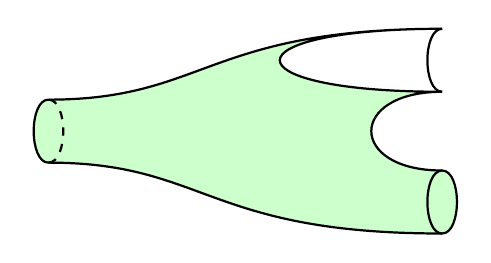
\begin{tikzpicture}[thick]
	\filldraw[fill=green!25, fill opacity=0.8]
	(1,2.6) .. controls (0.75,2.6) and (0.75,3.4) .. (1,3.4) .. 
	controls (3,3.4) and (3,4.3) .. (6,4.3) .. 
	controls (3.25,4.3) and (3.25,3.5) .. (6,3.5) .. 
	controls (4.8,3.5) and (4.8,2.5) .. (6,2.5) .. 
	controls (6.25,2.5) and (6.25,1.7) .. (6,1.7) ..
	controls (3,1.7) and (3,2.6) .. (1,2.6);
	\draw[dashed]
	(1,2.6) .. controls (1.25,2.6) and (1.25,3.4) .. (1,3.4);
	\draw  
	(6,4.3) .. controls (5.75,4.3) and (5.75,3.5) .. (6,3.5);
	\draw
	(6,2.5) .. controls (5.75,2.5) and (5.75,1.7) .. (6,1.7);
\end{tikzpicture}\]

\begin{ejem}
	El \textbf{cobordismo trivial} sobre $M$ es $W=M\times I$.
\end{ejem}

\begin{defn}
	Un cobordismo $W$ es un \textbf{h-cobordismo} si
	\[\begin{tikzcd}[row sep=tiny]
		\partial_-W\arrow[dr,hook]\\
		&W\\
		\partial_+W\arrow[ur,hook]
	\end{tikzcd}\]
\end{defn}
\begin{ejem}
	Los pantalones no lo son porque hay dos círculos que no pueden ser homotópicamente equivalentes. El coboridmo trivial sí lo es. El cobordismo trivial con un género no lo es, ya que el grupo fundamental de $W$ es libre no abeliano mientras las fronteras son círculos.
\end{ejem}

\begin{teo}[del h-cobordismo, Smale]
	Sea $W^m$ un h-cobordismo. Si $\pi_1(W)=1$ y $m\geq6$, entonces
	\[W^m\overset{\text{difeo}}{\approx}\partial_-W\times I\]
\end{teo}
El resto del curso estaremos demostrando esto, salvo la siguiente discusión, donde argumentamos por qué este teorema implica

\begin{teo}[Smale]
	$S^n\simeq M^n\implies S^n\approx M^n$ si $n\geq 6$ y $M^n$ es diferenciable.
\end{teo}
\begin{proof}
	A $M^n$ le quitamos dos discos $D^n$ para obtener el cobordismo $M=M-\{\int D^+\cup\int D^-\}$. De hecho,
	\begin{lema}
		$W$ es un h-cobordismo simplemente conexo.
	\end{lema}
	\begin{proof}
		Definamos las variedades
		\begin{align*}
			\mathcal{D}^+=W\cup D^+,\qquad\mathcal{D}^-=W\cup D^-
		\end{align*}
		Calculemos $H_i(\mathcal{D}^+)$ usando Mayer-Vietoris de acuerdo a que $M=\mathcal{D}^+\cup_{\partial_-W}D^-$.
		\[\begin{tikzcd}[column sep=small]
			 \cdots\arrow[r]&\tilde{H}_i(\partial_-W)\arrow[r]&\tilde{H}_i(\mathcal{D}^+)\oplus\tilde{H}_i(D^-)\arrow[r]&\tilde{H}_i(M)\arrow[r]&\tilde{H}_{i-1}(\partial_-W)\arrow[r]&\cdots
		\end{tikzcd}\]
		Así que $H_i(\mathcal{D}^+)=0$ salvo quizás para $i=n,n-1$ usando que $M$ es homotópicamente equivalente a una esfera.
		
		Por dualidad de Poincaré con frontera, $H_n(\mathcal{D}^+)\approx H^0(\mathcal{D}^+\partial_-W)$, $H_{n-1}(\mathcal{D})\approx H^i(\mathcal{D}^+,\partial_-W)$. Para calcular estas cohomologías de parejas hacemos la sucesión exacta de la pareja:
		\[\begin{tikzcd}
			0\arrow[r]&H^0(\mathcal{D}^+,\partial_-W)\arrow[r]&H^0(\mathcal{D}^+)\arrow[r]&H^0(\partial_-W)
		\end{tikzcd}\]
		Los últimos dos son $\Z$, lo que obliga a esa flecha a ser un isomorfismo y entonces $H^0(\mathcal{D}^+,\partial_-W)\approx0$. Continuando la sucesión,
		\[\begin{tikzcd}[column sep=small]
			0\arrow[r]&H^0(\mathcal{D}^+,\partial_-W)\arrow[r]&H^0(\mathcal{D}^+)\arrow[r]&H^0(\partial_-W)\arrow[r]&H^1(\mathcal{D}^+,\partial_-W)\arrow[r,hook]&H^1(\mathcal{D}^+)\arrow[r]&\cdots
		\end{tikzcd}\]
		Y $H^1(\mathcal{D}^+)\approx0$ por dualidad de poincaré ya que sabemos que los grupos de homología se anulan salvo en $i=n,n-1$. Es decir, $\tilde{H}_i(\mathcal{D}^\pm)=0$ para toda $i$.
		
		Para ver que $\mathcal{D}^\pm\approx1$ usamos Van Kampen en el mismo $M=\mathcal{D}^+\cup_{\partial_-W}D^-$ para obtener
		\[\pi_1(M)\approx\pi_1(\mathcal{D}^+)*_{\pi_1(\partial_-W)}\pi_1(D^-)\]
		Todos los que conocemos son triviales, así que el único que no conocemos, $\pi_1(\mathcal{D}^+)$ también es trivial. De manera análoga, Van Kampen nos dice que
		\[\pi_1(\mathcal{D}^+)\approx\pi_1(W)*_{\pi_1(S^{n-1})}\pi_1(D^+)\]
		así que $\pi_1(W)=1$.
		
		Finalmente veamos que $\partial_+W\hookrightarrow W$ es una equivalencia homotópica. Trataremos de aplicar Whitehead. Usaremos sin demostrar que como las variedades son diferenciables tienen una estructura CW. Busquemos una función entre ellas que induzca isomorfismos $f_*:H_i(Y)\to H_i(X)$ para toda $i$.
		
		Por Mayer-Vietoris una vez más,
		\[\begin{tikzcd}
			0\arrow[r]&H_i(\partial_+W)\arrow[r]&H_i(W)\oplus H_i(D^+)\arrow[r]&H_i(\mathcal{D}^+)\arrow[r]&\cdots
		\end{tikzcd}\]
		Y de hecho, $H_i(D^+)\approx H_i(\mathcal{D}^+)\approx0$.
	\end{proof}
	
	Entonces, por el teorema del h-cobordismo, $W\overset{\text{difeo}}{\approx}\partial_-W\times I\approx S^{n-1}\times I$. Así que tenemos un cilindro, le pegamos las tapas y terminamos: tenemos un homeomorfismo con $S^n$.
\end{proof}
\begin{obs}
	El homeomorfismo que construimos no necesariamente es un difeomorfismo. De hecho, qué bueno, porque como discutimos antes, Milnor probó que hay un contraejemplo en dimensión 7 para el caso difeomorfo.
	
	Es posible hacer que esta función sea un difeomorfismo salvo en un punto.
\end{obs}
Recordemos que
\begin{defn}\leavevmode
	\begin{enumerate}
		\item $f:M\to N$ es una \textbf{inmersión} si para todo $x\in M$, la diferencial $df_x:T_xM\to T_{f(x)}N$ es inyectiva.
		\item $f$ es un \textbf{encaje} si es una inmersión y $f:M\to f(M)$ es un homeomorfismo.
		\item Una \textbf{isotopía} es una función suave $F:M\times I\to N$ tal que
		\[f_t:=F(-,t):M\to N\]
		es un encaje para cada $t$.
	\end{enumerate}
\end{defn}

\begin{teo}[de extensión de isotopía]
	Si $f_t:M\to N$ es una isotopía, entonces existe otra isotopía
	\[F_t:N\to N\]
	tal que:
	\begin{enumerate}
		\item $F_0=\Id_N$
		\item $f_t=F_t\circ f_0$ para toda $t\in I$.
	\end{enumerate}
	es decir, podemos controlar una isotopía de $M$ en $N$ mediante una isotopía de $N$ en $N$.
\end{teo}

\begin{defn}
	El \textbf{asa} $h$ de dimensión $n$ e \textbf{índice} $I(h)$ $0\leq i\leq n$ es $D^i\times D^{n-i}\approx D^n$ donde $D^i=\{x\in\R^i:|x|\leq 1\}$.
\end{defn}
\begin{prop}
	\begin{align*}
	\partial h&=\partial D^i\times D^{n-i}\cup D^i\times \partial D^{n-i}\\
	&=\underbrace{S^{i-1}\times D^{n-i}}_{\partial^-h}\cup\underbrace{ D^{i}\times S^{n-(i+1)}}_{\partial^+h}
	\end{align*}
\end{prop}
\begin{ejem}
	Supongamos que $n=3$. Trataremos de dar una descomposición en asas que, a diferencia de una descomposición CW, todas las ``células" son de la misma dimensión, pero de índices distintos.
	\[\begin{matrix}
		i=0&i=1&i=2&i=3\\
		D^0\times D^3&D^1\times D^2&D^2\times D^1&D^3\times D^0
	\end{matrix}\]
	que parecen parecidos pero realmente no lo son, porque el $\partial^-h$ y el $\partial^+h$ cambian de papel.
\end{ejem}
Ahora consideremos $M^n$ una variedad con frontera, $h$ un asa de dimensión $n$ e índice $i$ y $f:\partial^-h\to\partial M$ un encaje. Definimos
\[M+h:=M\cup_f D^i\times D^{n-i}\]
que es una variedad diferenciable.

\begin{teo}
	Sea $M$ una variedad cerrada. Entonces $M$ admite una descomposición por asas, es decir,
	\[M\overset{\text{difeo}}{\approx} h_1+h_2+\ldots+h_r\]
	tal que $I(h_i)\leq I(h_{i+1})$.
\end{teo}
\begin{obs}
	La operación suma no es asociativa ni conmutativa. Se deben ir sumando una por una las asas.
\end{obs}

\begin{teo}
	Sea $W^n$ un cobordismo entre $\partial^-W$ y $\partial^+W$, entonces
	\[W^n=\partial^-W\times [0,1]+h_1+\ldots+h_m\]
	tal que $\partial^-W$ queda intacto en el sentido de que la imagen de ninguno de los encajes de pegado toca la tapa de abajo.
\end{teo}
Nuestro objetivo es desarrollar un mecanismo que a esta expresión nos permita quitarle un asa, de modo que terminaríamos iterando suficientes veces.

\section{Cálculo de asas}
\begin{lema}[1]
	Si $f,g:\partial^-h\to\partial h$ son isotópicos, entonces
	\[M+_fh\overset{\text{difeo}}{\approx}M+_gh\]
\end{lema}
\begin{proof}
	Consideramos
	\[f:\partial^-h\hookrightarrow \partial M\]
	\[F_t:\partial M\times I\to \partial M\]
	\begin{align*}
		F'_t:\partial M\times I&\to \partial M\times I\\
	(x,t)&\mapsto (F_t(),t)
	\end{align*}
	De donde, al considerar una vecindad regular de la frontera de $M$ obtenemos que el siguiente diagrama conmuta:
	\[\begin{tikzcd}
		\partial M\times I\arrow[d,"F'_t",swap]&h\arrow[l,swap,"f"]\arrow[d,"\Id"]\\
		\partial M\times I&h\arrow[l,swap,"g"]
	\end{tikzcd}\]
\end{proof}
En un asa
	\begin{align*}
	\partial h&=\partial D^i\times D^{n-i}\cup D^i\times \partial D^{n-i}\\
	&=\underbrace{S^{i-1}\times D^{n-i}}_{\partial^-h}\cup\underbrace{ D^{i}\times S^{n-(i+1)}}_{\partial^+h}
\end{align*}
diremos que $D^i\times\{0\}$ es el \textbf{disco de adjunción}, $S^{i-1}\times\{0\}$ es la \textbf{esfera de adjunción}. Correspondientemente, $\{0\}\times D^i$ es el \textbf{disco complementario} y $\{0\}\times S^{n-i-1}$ es la \textbf{esfera complementaria}.

Para un ejemplo tomemos $D^1\times D^2$. El disco de adjunción es el alma del cilindro, la esfera de adjunción son los centros de las tapas, el disco complementario es el disco a la mitad del cilindro y la esfera complementaria es la frontera del disco complementario.

Usaremos un resultado que Milnor de muestra con teoría de Morse. Damos una \textbf{descomposición por asas de $M$}. Tomamos una estructura de complejo CW en $M$. Declaramos que el 0-esqueleto sea una suma de 0-asas, $h^0_1+\ldots+h_{r_1}^0$. Para cada arista que une dos puntos consideramos una 1-asa que es un cilindro como en el párrafo anterior y extendemos nuestra estructura a $(h^0_1+\ldots+h_{r_0}^0)+(h^1_1+\ldots +h^1_{r_1})$.

\begin{teo}[De Whitehead]
	Hay una descomposición por asas de $M$
	\[(h^0_1+\ldots+h_{r_0}^0)+(h^1_1+\ldots +h^1_{r_1})+\ldots\]
\end{teo}
Si $W$ es un cobordismo entre $\partial^-W$ y $\partial^+W$, consideramos
	\[W^n=\partial^-W\times [0,1]+(h^0_1+\ldots+h_{r_0}^0)+(h^1_1+\ldots +h^1_{r_1})+\ldots\]
Y de nuevo, nuestro objetivo es quitar las asas una por una.

A partir de ahora el símbolo $=$ signifca difeomorfismo.
\begin{lema}[2]
	$(M+h_1)+h_2$. Sea $N=\partial(M+h_1)$. Denotemos or $S$ a la esfera complementaria de $h_1$ y $\mathcal{S}$ la esfera de adjunción de $h_2$. (Notemos que  $S$ y $\mathcal{S}$ son subvariedades de $N$.) Si $S$ y $\mathcal{S}$ son disjuntas, entonces (módulo isotopía), puedo adjuntar $h_1$ y $h_2$ al mismo tiempo, es decir,
	\[(M+h_1)+h_2=M+(h_1\sqcup h_2)\]
\end{lema}
\begin{proof}
	Si las funciones de pegado no se tocan, terminamos. Si, en cambio, pego una asa y luego otra, y la segunda se pega sobre la primera, al menos sabemos que las esferas de adjunción no se tocan. Pero sí se podrían tocar partecitas del asa alrededor de $\mathcal{S}$, pero no importa, porque puedo isotopear, aplicando el lema 1, a un asa que no toca la esfera de adjunción de la primera asa, $S$. Y finalmente, podemos isotopear la segunda asa hasta que no toque en lo absoluto a la primera asa.
\end{proof}

Ahora consideremos dos asas con índices consecutivos, digamos $I(h_1)=i$, $I(h_2)=i+1$. Entonces la esfera complementaria $S$ de $h_1$ tiene dimensión $n-i-1$ y la esfera de adjunción $\mathcal{S}$ de $h_2$ tiene dimensión $n-i$. Sus codimensiones son $i+1$ y $n-i$ respectivamente, suya suma es $n-1$ y por el teorema de transversalidad, $\dim(S\cap \mathcal{S})=0$.

De ahora en adelante supondremos que la esfera complementaria de un asa y la esfera de adjunción de un asa se intersectan transversalmente. La descomposición de $M$ dada de esta forma se llama \textbf{descomposición t-estándar}.

Ahora enunciamos el lema que nos permite quitar asas.

\begin{lema}[3]
	Dadas dos asas de índices consecutivos $I(h_1)=i$, $I(h_2)=i+1$, si $S\cap\mathcal{S}$ es exactamente un punto, entonces $M+h_1+h_2=M$.
\end{lema}
\begin{proof}
	(del lema 3). Consideremos primero adjuntar una 0-asa, es decir, una bola. La esfera de adjunción es un punto y la complementaria una esfera, de hecho el resultado es algo disconexo. Ahora adjuntamos una 1-asa. El resultado es equivalente a adjuntar una bola. Realmente no modificamos la variedad.
	
	Ahora comencemos por adjuntar una 1-asa. Obtenemos literalmente un asa como de una tasa pegada a la variedad, cuya esfera de adjunción es un círculo a la mitad del asa. Ahora adjuntamos una 2-asa. Podemos suponer que la esfera de adjunción se ve como una línea longitudinal sobre la primera asa, y en el resto de la variedad puede ser muy exótica. Y el resto de la segunda asa, de hecho, rellena el hoyo o ``género" que se había formado al pegar la primera asa.
	
	El paso final es demostrar que este proceso se puede ver como pegar tres asas, que a la mera hora es equivalente a pegar una bola.
\end{proof}

Para terminar nuestra demostración basta ver que en una descomposición t-estándar de $M$ podemos encontrar para cada $i$-asa una $(i+1)$-asa cuyas esferas complementaria y de adjunción se intersecten en exactamente un punto.

\begin{defn}
	Sean dos asas de índices consecutivos $I(h_1)=i$, $I(h_2)=i+1$. Supongamos que $2\leq I(h_1)\leq n-3$, que $n\geq6$ y que $\pi_1(N)=0$. $N$, $S$ y $\mathcal{S}$ son orientables, así que podemos fijar una orientación para cada una. La intersección $S\cap\mathcal{S}$ es una cantidad finita de puntos, a los que podemos asignar un número $\pm1$, dependiendo de la orientación. El \textbf{\textit{número de intersección orientado}} es
	\[\sum_{s\in S\cap \mathcal{S}}\sigma(x)=\pm1\]
\end{defn}
\begin{lema}[4, el truco de Whitney]
	En la situación anterior, podemos isotopear $\mathcal{S}$ de forma que $S\cap \mathcal{S}$ es un punto.
\end{lema}
\begin{proof}
	Tomamos curvas que unen una pareja de puntos en $S\cap \mathcal{S}$. Por ser simplemente conexo, podemos considerar el espacio entre las curvas como un disco. Para isotopear esta inmersión a un encaje, necesitamos dimensión al menos 6.
\end{proof}
En consecuencia,
\[M+h_1+h_2=M\]
%Ahora queremos encontrar dos asas que se cancelan.
Definamos $C_i$ como el grupo abeliano libre generado por las asas de índice $i$ y el siguiente complejo de cadenas:
\[\begin{tikzcd}
	C:C_n\arrow[r,"D^n"]&C_{n-1}\arrow[r,"D^{n-1}"]&\cdots\arrow[r]&C_1\arrow[r,"D^1"]&C_0\arrow[r]&0
\end{tikzcd}\]
donde
\[D_{k,j}^i=\sum_{S_j\cap\mathcal{S}_k}\sigma(x)\]
para $S_j$ la esfera complementaria de $h_j^i$ y $\mathcal{S}$ es la esfera de adjunción de $h^{i+1}_k$.
%\[\begin{matrix}
%	0\cdots&
%\end{matrix}\]
\begin{prop}
	$C$ es un complejo de cadenas y $H_\bullet(C)\approx H_\bullet(W,\partial^-W)$.
\end{prop}
Notemos que si $W$ es un h-cobordismo, $\partial^-W\subset W$ es una equivalencia homotópica, y por la sucesión exacta larga de la pareja $H(W,\partial^-W)$ se hace cero. En conclusión, el complejo de cadenas $C$ es acíclico.

\begin{lema}[5]
	Fijemos $0\leq j,k\leq m_i$ y $(h_j^i,h_k^i)$ asas. Entonces, podemos construir otra descomposición por asas de $W$ tal que es t-estándar y tal que
	\begin{itemize}
		\item Tiene el mismo número de asas en cada índice.
		\item Las matrices de incidencia son iguales salvo la de índice $i$.
	\end{itemize}
			La nueva matriz de incidencia, $\mathcal{D}^i$ de $D^i$ se obtiene a través de la operación elemental de sumar (o restar) la $k$-ésima columna a la $j$-ésima columna.
\end{lema}
\begin{prop}
	Si $W$ es un h-cobordismo de dimensión $\geq6$, $W$ admite una descomposición por asas t-esándar sin asas de índices $0,1, n-1,n$.
\end{prop}

\begin{proof}
	(del teorema del h-cobordismo). Sólo debemos encontrar dos asas que se puedan cancelar. Comencemos con una descomposición por asas como en la proposición anterior, digamos
	\[W=\partial^-W\times I\times h_1\times\ldots\times h_m\]
	y consideremos su complejo de cadenas asociado. Sea $i-1$ tal que $C_{i-1}$ es el primer grupo no cero.
	\[\begin{tikzcd}
		\cdots\arrow[r]&C_i\arrow[r,"D^i"]\arrow[r]&C_{i-1}\arrow[r]&0\arrow[r]&\cdots\arrow[r]&0
	\end{tikzcd}\]
	Como $W$ es un h-cobordismo, $H_\bullet(C)=0$. En particular, $D^i$ es suprayectiva. Así, podemos ``diagonalizar" la matriz para obtener algo de la forma
	\[\left(\begin{matrix}
		\pm1&0&\cdots &0\\
		0&\pm1\\
		\vdots&&\\
		0&&\cdots&\pm1
	\end{matrix}\right)\]
	Es posible construir complejo de cadenas usando el lema 5 cuya $D^i$ es exactamente esta matriz. Esto hace que el número de intersección de $S_j\cap\mathcal{S}_k$ sea $\pm1$.
	
	Si en la expresión
	\begin{align*}
		W=\partial^-W\times[0,1]+&({\color{blue}h_1^{i-1}}+\ldots+h_{m_{i-1}}^{i-1})\\
		&+({\color{blue}h_1}^i+\ldots+h^i_{m_{i}})+\ldots
	\end{align*}
	Y si logramos poner los términos azul en orden consecutivo, podríamos cancelarlos. Usando el lema 5, la expresión anterior es
	\begin{align*}
		=\partial^-W\times[0,1]+&(h_2^{i-1}\sqcup\ldots\sqcup h^{i-1}_{m_i-i}\sqcup {\color{blue}h_1^{i-1}})\\
		&+({\color{blue}h_{m_i}^i}\sqcup h_1^i\sqcup\ldots\sqcup h_{m_i-1}^i)+\ldots
	\end{align*}
	Y para cancelar las asas sólo debemos confirmar la hipótesis de ser simplemente conexo. Por hipótesis tenemos que $W$ es simplemente conexo, así que $W\times[0,1]$ también. Y luego, para $i-1\leq2$, también
	\[\pi_1(W\times[0,1]+h_2^{i-1})=1\]
	Entonces, en la expresión anterior podemos descartar los términos en azul. Y nada, podemos iterar el proceso.
\end{proof}

\clearpage
\chapter{Exposiciones}
\section{$K$-teoría}
\begin{defn}\leavevmode
	\begin{itemize}
		\item Un \textbf{\textit{fibrado}} o \textbf{\textit{haz}} vectorial es una función $p:E\to B$ tal que
	\begin{enumerate}
		\item Para todo $b\in B$, $p^{–1}(b)$ es un espacio vectorial (sobre $\R$ o $\C$).
		
		\item Existe un cubrimiento $(U_\alpha)$ por abiertos de $B$ tal que $p^{-1}\approx U\times\R^n$ es un homeomorfismo
	\end{enumerate}
	\item Un \textbf{\textit{morfismo}} de fibrados vectoriales es una función que hace conmutar el siguiente diagrama
	\[\begin{tikzcd}
		E_1\arrow[rr]\arrow[dr,swap,"p_1"]&&E_2\arrow[dl,"p_2"]\\
		&B
	\end{tikzcd}\]
	\item El \textbf{\textit{pullback}} de un haz vectorial es
	\[\begin{tikzcd}
		E'\arrow[r]\arrow[d,swap,"p'"]&E\arrow[d]\\
		X\arrow[r,"f"]&Y
	\end{tikzcd}\]
	que resulta en una flecha $\operatorname{Vect}(Y)\to\operatorname{Vect}(X)$.
	\end{itemize}
\end{defn}
\begin{lema}
	En la siguiente situación
	\[\begin{tikzcd}
		E_1\arrow[rr,"f"]\arrow[rd,swap,"p_1"]&&E_2\arrow[ld,"p_2"]\\
		&B
	\end{tikzcd}\]
	$f$ es un isomorfismo si $f|_{p^{-1}(b)}$ es un isomorfismo lineal en cada fibra.
\end{lema}

\begin{defn}
	La \textbf{\textit{suma directa}} de dos fibrados vectoriales
	\[\begin{tikzcd}
		E_1\arrow[rd,swap,"p_1"]&&E_2\arrow[ld,"p_2"]\\
		&B
	\end{tikzcd}\]
	es $E_1\oplus E_2:=\{(e_1,e_2):p(e_1)=p(e_2)\}\subset E_1\times E_2$.
\end{defn}

\begin{obs}\leavevmode
	\begin{itemize}
		\item Si $\varepsilon^n$ denota el haz trivial de dimensión $n$, tenemos que $\varepsilon^n\oplus \varepsilon^m=\varepsilon^{n+m}$.
		
		\item Si $B$ es Housdorff compacto, para cualquier haz vectorial $E\to B$, existe otro $E'\to B$ tal que $E\oplus E'$ es trivial.
		\[\begin{tikzcd}
			E\arrow[d]&E'\arrow[ld]\\
			B
		\end{tikzcd}\]
	\end{itemize}
\end{obs}

\begin{defn}
	El \textbf{\textit{producto tensorial}} de dos haces como en la definición de suma directa es $E_1\otimes E_2:=\bigsqcup p_1^{-1}(b)\otimes p_2^{-1}(b)$. Para darle una topología tomemos $U\subset B$ tal que $p^{-1}_1(U)\overset{\varphi_1}{=}\R^n\times U$ y $p^{-1}_2(U)\overset{\varphi_2}{=}\R^m\times U$, y requerimos que
	\[\varphi_1\otimes\varphi_2:p^{-1}_1(U)\otimes p_2^{-1}(U)\to U(\R^n\otimes\R^m)\]
	sea un homeomorfismo.
\end{defn}

Ahora, en $\operatorname{Vect}(X)$,
\begin{itemize}
	\item $E_1\approx E_2$ si y sólo si existen $n,m$ números naturales tales $E_1\otimes\varepsilon^n\simeq E_2\otimes\varepsilon^m$.
	
	\item $E_1\sim E_2$ si y sólo si existe $n$ tal que $E_1\oplus \varepsilon^n\simeq E_2\oplus \varepsilon^n$.
\end{itemize}


	El \textbf{\textit{grupo de categoría de $X$ reducido}} $\tilde{K}(X)$ como el grupo $(\operatorname{Vect}(X)/\sim ,\oplus)$. Observemos que la relación $\approx$ no tiene inversos. Para construir un grupo, los agregamos mediante $(E_1-E_2)=(E_1'-E_2')$, $E_1+E_2'=E_2+E_1'$ y $(E_1-E_2)\oplus(E_1'-E_2')=(E_1\oplus E_1)-(E_1'\oplus E_2')$. Con esto tenemos $K(X)$, el \textbf{\textit{grupo de categoría de $X$}}.
	
	Dada $X\overset{f}{\to}Y$ tenemos el pullback $\tilde{K}(Y)\overset{f^*}{\to}\tilde{K}(X)$. Y también está
	\begin{align*}
		K(X)&\overset{\varphi}{\to}\tilde{K}(X)\\
		E-\varepsilon^n&\mapsto [E]_\sim
	\end{align*}
	cuyo kernel es $\ker(\varphi)=(\varepsilon^m-\varepsilon^n)$
	Luego
	\begin{align*}
		K(X)\overset{\psi}{\to}K(\{x_0\})
	\end{align*}
	con $\ker(\psi)=p^{-1}(x_0)$. Notemos que le grupo de categoría de un punto es los enteros:
	\[\begin{tikzcd}
		E'\arrow[r]\arrow[d]&E\arrow[d]\\
		\{x_0\}\arrow[r,"i"]&X
	\end{tikzcd}\]
	donde $E'=\{(e,x_0):p(e)=x_0\}$. Y también, $\ker(K(X)\to K(\{x_0\}))=\tilde{K}(X)$.

Ahora le damos estructura de anillo a $K(X)$. Dado
	\[\begin{tikzcd}
	E_1\arrow[rd,swap,"p_1"]&&E_2\arrow[ld,"p_2"]\\
	&B
\end{tikzcd}\]
tenemos $\tilde{K}(X)=\ker(K(X)\to K(x_0))$. Y definimos el producto externo
\begin{align*}
	\sigma:K(X)\otimes K(Y)&\to K(X\times Y)\\
	a\otimes b&\mapsto p_1^*(a)p_2^*(b)
\end{align*}
Ahora usaremos el \textbf{\textit{fibrado vectorial línea}}, que está dado en $H\subseteq \C P^1\times \C^2=\{(x,y):v\in x\}$ como
\[\begin{tikzcd}[column sep=tiny]
	H\arrow[d,swap,"p"]&(x,v)\arrow[d,maps to]\\
	\C P^1&x
\end{tikzcd}\]
\begin{af}
	$(H\otimes H)\oplus1=H\oplus H$
\end{af}
\begin{teo}[Fundamental del producto]
	De acuerdo a composición
	\[\begin{tikzcd}
			\Z[H]/(H-1)^2\otimes K(X)\arrow[r]&K(S^2)\otimes K(X)\arrow[r]&K(S^2\times X)
	\end{tikzcd}\]
	hay un isomorfismo
	\[\Z[H]/H-1\to K(S^2)\]
\end{teo}

Ahora estudiemos las sucesiones exactas.
Para 
\[\begin{tikzcd}
	A\arrow[hook,r,"i"]&X\arrow[r,"q"]&X/A
\end{tikzcd}\]
tenemos
\[\begin{tikzcd}
	\tilde{K}(X/A)\arrow[r,"q^*"]&\tilde{K}(X)\arrow[r,"i^*"]&\tilde{K}(A)
\end{tikzcd}\]
Tomando conos y suspensiones,
\[\begin{tikzcd}[column sep=small]
	A\arrow[r,hook]&X\arrow[r,hook]&X\cup CA\arrow[r]\arrow[d]&(X\cup CA)\cup CX\arrow[d]\arrow[r]&((X\cup CA)\cup CX)\cup C(X\cup CA)\arrow[d]\\
	&&X/A&SA&SX
\end{tikzcd}\]
\begin{lema}
	Si $A$ es contráctil, entonces $q:X\to X/A$ induce una biyección $\operatorname{Vect}(X/A)\to\operatorname{Vect}(X)$.
\end{lema}
Y por fin tenemos la sucesión exacta
\[\begin{tikzcd}[column sep=small]
	\cdots\arrow[r]&\tilde{K}(S(X/A))\arrow[r]&\tilde{K}(SX)\arrow[r]&\tilde{X}(SA)\arrow[r]&\tilde{K}(A/X)\arrow[r]&\tilde{K}(X)\arrow[r]&\tilde{K}(A)
\end{tikzcd}\]
\begin{teo}[De periodicidad de Bott]
	\[\tilde{K}(X)\simeq\tilde{K}(S^2X)\]
	donde $S^2X$ es la doble suspensión de $X$.
\end{teo}
\begin{coro}
	\[\tilde{K}(S^n)=\begin{cases}
		\Z\qquad\text{ si }n\text{ es par}\\
		0\qquad\text{ si }n\text{ es impar}
	\end{cases}\]
\end{coro}

Ahora veamos aplicaciones de esto:
\begin{defn}
	$S^n$ es \textbf{\textit{paralelizable}} si existen campos vectoriales $V_1,\ldots,V_n$ tales que $\{V_1,\ldots,V_n\}$ es linealmente independiente en cada punto de $S^n$. Esto es equivalente a que el haz tangente sea trivial.
\end{defn}

\begin{teo}
	Sólo $n=1,2,4,8$ cumplen lo siguiente:
	\begin{enumerate}
		\item $\R^n$ es un álgebra de división.
		\item $S^{n-1}$ es paralelizable.
	\end{enumerate}
\end{teo}

\textcolor{cyan}{¿Qué nos dice el hecho de que el haz tengente sea trivial respecto a la curvatura? $S^1$ es plana en el sentido de Lee, ie. localmente isométrica al espacio euclideano.}

\begin{defn}
	$S^{n-1}$ es un \textbf{\textit{H-espacio}} si existen $S^{n-1}\times S^{n-1}\overset{H}{\to} S^{n-1}$ y $e\in S^{n-1}$ tales que $H(e,x)=x=H(x,e)$.
\end{defn}

\begin{prop}
	Si $n$ satisface alguna de las consecuencias del teorema anterior, entonces $S^{n-1}$ es un H-espacio.
\end{prop}
\begin{proof}\leavevmode
	\begin{enumerate}
		\item $(x,y)\to xy/|xy|$
		\item Para cada $x\in S^{n-1}$ tomamos una base ortonormal. Podemos decidir que la base correspondiente a $e_1$ sea la base canónica de $\R^{n-1}$. Luego tomamos $\alpha_x\in\operatorname{SO}(n)$ que convierte la base en $x$ en la canónica. El mapeo $(x,y)\mapsto \alpha_x(y)$ es el buscado.
	\end{enumerate}
\end{proof}
\begin{obs}\leavevmode
	\begin{enumerate}
		\item $\tilde{K}(S^{2n})=\Z$ y $\tilde{K}(S^{2n+1})=0$.
		\item $\tilde{K}(S^{2k})\otimes \tilde{K}(X)\to\tilde{K}(S^{2k}\cap X)$
		\item $K(S^{2k})\otimes K(X)\to K(S^{2k}\times X)$ es un isomorfismo.
	\end{enumerate}
\end{obs}
	De lo cual se sigue $S^{2k}$ no es un H-espacio si $k>0$. Resta demostrar que los únicos casos donde $S^{n-1}$ es un H-espacio son $2,4$ y $8$.
	
	\section{Clases características}
	Consideremos una matrix
	\[X=\begin{pmatrix}
		x&y\\
		z&w
	\end{pmatrix}\]
	\begin{defn}
		$P(X)$ se llama \textbf{$\operatorname{GL}(r,X)$-invariante} si para cualquier matriz $A\in\operatorname{GL}(r,\R)$
		\[P(A^{-1}XA)=P(X)\]
	\end{defn}
	\begin{ejem}\leavevmode
		\begin{enumerate}
			\item $\det(X)$. Para $X$ definida arriba, $\det(X)=xw-yz$
			\item $\operatorname{tr}(X)$. Para $X$ definida arriba, $\operatorname{tr}(X)=x+w$
			\item $\det(\lambda I+X)$. Para $X$ en general, $\det(\lambda I+X)=\lambda^r+f_1(X)\lambda^{r-1}+\ldots+f_r(X)$.
			\item $\operatorname{tr}_k(X)=\operatorname{tr}(X^k)$.
		\end{enumerate}
	\end{ejem}
	
	\begin{prop}
		Si $\mathcal{A}$ es $\R$-álgebra conmutativa con unidad y $P$ es $\operatorname{GL}$-invariante, entonces para una matriz con entradas en $\mathcal{A}$, digamos $X\in\mathcal{A}(X^i_j)$,
		\[P(A^{-1}XA)=P(X)\qquad \text{para }A\in\operatorname{GL}\]
	\end{prop}
\begin{defn}
	Sea $E\to M$ un haz vectorial sobre $M$. Una \textbf{\textit{conexón}} en $E$ es una función
	\[\nabla:\Gamma(TM)\times\Gamma(E)\to \Gamma(E)\]
	tal que para todo $X\in\Gamma(TM)$ y $s\in\Gamma(E)$,
	\begin{enumerate}
		\item $\nabla_Xs$ es $C^\infty(M)$-bilineal.
		\item $\nabla_Xs$ satisface la regla de Leibniz en $s$: para $f\in C^\infty(M)$,
		\[\nabla_X(fs)=(Xf)s+f\nabla_Xs\]
	\end{enumerate}
\end{defn}
\begin{defn}
	El \textbf{tensor de curvatura} en una variedad es una función $\R$-multilineal
	\[R:\Gamma(TM)\times\Gamma(TM)\times\Gamma(s)\to\Gamma(s)\]
	dada por
	\[R(X,Y)s=\nabla_X\nabla_Y s-\nabla_Y\nabla_Xs-\nabla_{[X,Y]}s\]
\end{defn}
Dado un marco local $e_1,\ldots,e_k$ en $U$,
\[R(X,Y)e_j=\sum\Omega_j^i(X,Y)e_i\]
donde $\Omega=(\Omega^j_i)$ es una matriz de 2-formas.

Veamos que esta matriz está bien definida cuando cambiamos de marco. Sea $\tilde{e}_1,\ldots,\tilde{e}_n$ otro marco local en $U$. Entonces hay una función $a:U\to\operatorname{GL}(k,\R)$ tal que $\tilde{\Omega}=a\Omega a^{-1}$.

Ahora tratemos de definir el morfismo de Chern-Weil. Sea $P$ un polinomio homogéneo de grado $k$ $\operatorname{GL}$-invariante y $p\in M$. Consideremos 
\[\mathcal{A}=\bigoplus_{i=0}^\infty \bigwedge^{2i}(T^*_pM)\]
Observemos que $\Omega_p\in \mathcal{A}$. Por la invarianza de $\Omega$ bajo conjugación, tenemos que $P(\Omega_p)=P(\tilde{\Omega}_p)$.
	
Cuando dejamos variar $p$ sobre la variedad, obtenemos una función $P(\Omega):U\to\bigwedge$.

Por ejemplo,
\[P(\Omega)=\left|\begin{matrix}
	\Omega^1_1&\Omega^2_1\\
	\Omega^1_2&\Omega^2_2
\end{matrix}\right|=\Omega^1_1\wedge\Omega^2_2-\Omega^2_1\wedge\Omega^1_2\in\bigwedge^4(T^*M)\]

Así que en general $P(\Omega)\in\bigwedge^{2k}(M)$.
\begin{teo}
	$P(\Omega)$ es una forma cerrada y $[P(\Omega)]_{dR}$ no depende de $\nabla$.
\end{teo}

Hasta ahora hemos construido un mapeo
\[\left\{\text{polinomios homogéneos invariantes}\right\}\longrightarrow H^*(M)\]
Y quisiéramos extenderlo a todos los polinomios invariantes. De hecho, $\operatorname{Inv}(\operatorname{GL}(r,\R))$ está generado por cualquiera de los siguientes conjuntos:
\begin{enumerate}
	\item $\{f_i(X)\}$.
	\item $\{\operatorname{tr}_k(X)\}$.
\end{enumerate}
Así que de hecho tenemos
\[\left\{\text{polinomios invariantes}\right\}\overset{CE}{\longrightarrow} H^*(M)\]
mediante
\[C_E(PQ)=[P(\Omega)\wedge Q(\Omega)]\]
Ahora podemos definir
\begin{defn}
La \textbf{clase de Pontrjiagin} es:
	\[P_k(E)=C_E\left(f_{2k}\left(\frac{1}{2\pi}\Omega\right)\right)\in H^{4k}(M)\]	
\end{defn}
Para definir la clase de Euler, necesitaremos
\begin{prop}
	Si $X$ es una matrix de $2m\times 2m$ antisimétrica, entonces $\det(X)$ es un cuadrado perfecto en $\Z(x^i_j)$.
\end{prop}
\begin{defn}
	El polinomio \textbf{Pfaffiano} es $\operatorname{Pf}(X)=\sqrt{\det(X)}$.
\end{defn}
que no es invariante en todo $\operatorname{GL}(r,\R)$, pero sí en $\operatorname{SO}(r,\R)$. Ahora sí,
\begin{defn}
	La \textbf{clase de Euler} es
	\[e(E)=c_E(\operatorname{Pf}(X))\]
\end{defn}
\begin{teo}
	Si $M$ es compacta, riemanniana de dimensión para y orientable, entonces
	\[\int_M\operatorname{Pf}(\Omega)=\chi(M)\]
\end{teo}
\begin{defn}
	En el polinomio
	\[\det(I+\frac{i}{2\pi}\Omega)=1+c_1(E)+\ldots+c_r(E)\]
	 los términos $c_i(E)$ son las \textbf{clases de Chern-Weil}.
\end{defn}

Finalmente podemos dar una interpretación funtorial de las clases características. Para
\[\operatorname{Vect}_k(M)=\{[E\overset{\pi}{\to}M]_{\simeq}:\dim(E)=k\}\]
tenemos
\[\operatorname{Vect}_k(-)\to H^*(-)\]
que es natural en cuanto a que para una flecha $M\to N$,
\[\begin{tikzcd}
	f^*E\arrow[r]\arrow[d]&E\arrow[d]\\
	M\arrow[r,"f"]&N
\end{tikzcd}\]
conmuta.

Ahora veamos una aplicación:
\begin{prop}
	Si $M$ es compacta de dimensión $4m$ y $M\hookrightarrow \R^{4m+1}$ es una hipersuperficie, entonces $P_k(M)$ se anula.
\end{prop}

\begin{defn}
	Una \textbf{variedad de Calabi-Yau} es una variedad compleja, de Käler, compacta y con primera clase de Chern cero.
\end{defn}
Recordemos cómo se define la característica de Euler:
\[\chi(M)=\sum_i(-1)^ic_n=\sum_i(-1)^i\beta_n\]
donde $c_n$ es una $n$-célula y $\beta_n=\operatorname{ran}H_n$.

\begin{teo}
	Si $V_1:M\to TM$ es un campo con ceros aislados, entonces
	\[\chi(M)=\sum\text{ceros de }V_1\]
\end{teo}
Cuya generalización es que
\begin{teo}
	Si $V_1,\ldots,V_k:M\to TM$, entonces $\{p\in M:\det(V_{ip})=0\}$ es una subvariedad de dimensión $k-1$ que define un $\Z_2$-ciclo.
\end{teo}
Para dar un ejemplo de cómo usar las clases características trataremos de dar una generalización del teorema de la bola peluda en el caso de los espacios proyectivos. Veremos en qué casos existen campos \textbf{\textit{paralelizables}}.

Dado un haz $E\overset{\pi}{\to}M$, hay una sucesioón $\{w_i(\pi):i\in\N\}$ con $w_i(\pi)\in H^i(M,\Z_2)$ tal que
\begin{itemize}
	\item $w_0(\pi)=1$
	\item $w_i(\pi)=0$ para $i>0$.
	\item (Naturalidad.) Si $f:B(\varepsilon)\to B(\eta)$ continua (o diferenciable) induce una función $f^*:H^2(B(\eta),\Z_2)\to H^i(B(\varepsilon),\Z_2)$ dada por $w_i(\eta)\mapsto w_i(\varepsilon)$.
	\item (Regla del producto de Whitney). $w_k(\varepsilon\oplus\eta)=\sum_{i=0}^kw_i(\varepsilon)\smile w_{k-i}(\eta)$.
	\item Un haz de línea $\gamma_1^1\to p^1$, $w_1(\gamma^1_1)$.
\end{itemize}
\begin{prop}
	Si $\eta\approx\varepsilon$ entonces $w_i(\eta)=w_i(\varepsilon)$.
\end{prop}
\begin{proof}
	Recordemos que dos haces sobre el mismos espacio son isomorfos si hay un diagrama conmutativo
	\[\begin{tikzcd}
		E(\eta)\arrow[r]\arrow[d,"\eta"]&E(\varepsilon)\arrow[d]\\
		M\arrow[r,swap,"1"]&M
	\end{tikzcd}\]
	De forma que nos basta probar naturalidad, y de hecho
	\begin{align*}
		1^*:H^i(M,\Z_2)&\to H^i(M,\Z_2)\\
		w_i(\varepsilon)&\mapsto w_i(\eta)
	\end{align*}
\end{proof}

\begin{prop}
	Si $\varepsilon\to M$ es trivial, $w_i(\varepsilon)=0$ para $i>0$.
\end{prop}
\begin{proof}
	Tenemos
	\[\begin{tikzcd}
		E(\varepsilon)\arrow[r,"\approx"]\arrow[d]&M\times\R^k\arrow[d]&\{\cdot\}\times\R^k\arrow[l,swap,hook]\arrow[d]\\
		M\arrow[r,swap,"1"]&M&\{\cdot\}\arrow[l,swap,hook]
	\end{tikzcd}\]
	y el mapeo inducido manda la cohomología al cero.
\end{proof}
\begin{prop}
	Si $\varepsilon$ es trivial, entonces $w_j(\varepsilon\oplus\eta)=w_j(\eta)$.
\end{prop}
\begin{proof}
	Directo de la regla de Whitney,
	\begin{align*}
		w_k(\varepsilon\oplus\eta)&=\sum_{i=0}^kw_i(\varepsilon)\smile w_{k-i}(\eta)\\
		&=w_0(\varepsilon)\smile w_k(\eta)\\
		&=w_k(\eta)
	\end{align*}
\end{proof}
\begin{prop}
	Si $\eta$ tiene dimensión $n$ y métrica $\mu:M\to\R$, y tiene una sección que no se anula, $w_n(\eta)=0$.	
\end{prop}
\begin{proof}
	Tomemos una sección $X:B(\eta)\to E(\eta)$ que no se anula. Podemos descomponer la fibra, que es un espacio euclideano para obtener $\tilde{X}\oplus\tilde{X}^\perp\equiv\eta$. Como $\tilde{X}$ es trivial, $w_n(\tilde{X}\oplus\tilde{X}^\perp)=w_n(\tilde{X}^\perp)=0$.
\end{proof}
\begin{coro}
	Si tenemos $X_1,\ldots,X_k$ secciones globales linealmente independientes que no se anulan, entonces $0=w_n(\eta)=w_{n-1}(\eta)=\ldots=w_{n-k+1}(\eta)$.
\end{coro}
\begin{obs}
	Una variedad es paralelizable (si haz tangente es trivial) si $w(M)=1$.
\end{obs}
\begin{defn}
	La \textbf{\textit{clase total de Stiefel-Whitney}} de un haz vectorial trivial $\xi$ de dimensión $n$ sobre $B$ es
	\[w(\xi)=1+w_1(\xi)+w_2(\xi)\ldots+w_n(\xi)+0+\ldots\]
\end{defn}
Para abordar el ejemplo que tenemos en mente, dado un haz lineal sobre el proyectivo, calculamos $w(\gamma^1_n\to P^n)$. Tenemos $E(\gamma^1_n)\subset P^n\times\R^{n+1}$.
\[\begin{tikzcd}
	E(\gamma^1_1)\arrow[r]\arrow[d]&E(\gamma^1_n)\arrow[d]\\
	P^1\arrow[r,hook,"i"]&P^n
\end{tikzcd}\]
Que inducen
\begin{align*}
	H^1(P^n,\Z_2)&\overset{i^*}{\to}H^1(P^1,\Z_2)\\
	w_1(\gamma^1_n)&\mapsto w_1(\gamma^1_1)=1
\end{align*}
usando que el producto copa del elemento no trivial en la cohomología del proyectivo va a dar al elemento no trivial. Luego,
\[w(\gamma^1_n)=(1+a)+0+0+\ldots\]
Además, tenemos
\[\gamma^1_n\oplus\gamma^\perp\approx P^n\times\R^{n+1}\]
y de hecho
\[w(\gamma^\perp)=1+a+\ldots+a^n\]
donde $a^k=a\smile\ldots\smile a$.

Luego, Milnor y Sheffel prueban que
\[TP^n\approx \Hom(\gamma^1_n,\gamma^\perp)\]

\begin{teo}
	\[TP^n\oplus(P^n\times\R)\approx\underbrace{\gamma^n\oplus\ldots\oplus\gamma^1_n}_{n+1\text{ veces}}\]
\end{teo}
\begin{proof}
	\[TP^n\oplus(P^n\times\R)\approx\Hom(\gamma^1_n,\gamma^\perp)\oplus (P^n\times\R)\]
	y de hecho
	\begin{align*}TP^n\oplus(P^n\times\R)&\approx\Hom(\gamma^1_n,\gamma^\perp)\oplus\Hom(\gamma^1_n,\gamma^1_n)\\
		&\approx\Hom(\gamma^1_n,\gamma^1_n\oplus\gamma^\perp)\\
		&\approx(\gamma^1_n,P^n\times\R^{n+1})\\
		&\approx\Hom(\gamma^1_n,P^n\times\R)\oplus\ldots\oplus\Hom(\gamma^1_n,P^n\times\R)\\
		&\approx\underbrace{\gamma^1_n\oplus\ldots\oplus\gamma^1_n}_{n\text{ veces}}
	\end{align*}
	así que 
	\begin{align*}
		w(TP^n)&= w(\gamma^1_n\oplus\ldots\oplus\gamma^1_n)\\
		&=w(\gamma^1_n)\ldots w(\gamma^1_n)\\
		&=(1+u)^{n+1}
	\end{align*}
\end{proof}
Por fin, como vimos en el curso, $w(TP^n)=1\iff n+1=2^k$.

¿Cuáles podrían ser paralelizables? $P^1$, $P^3$, $P^7$, $P^{15}$, $P^{31}$.

De hecho, podemos construr campos paralelos en $S^1$, $S^3$, $S^7$ y $S^{15}$ usando las estructuras de cuaternios, octonios, etc, que descienden al proyectivo. De hecho, a partir de 15 no es posible.

\section{Teorema de de Rham vía cohomología de gavillas}
\begin{defn}\leavevmode
\begin{itemize}
	\item 	Sea $X\in\operatorname{Top}$ y $\mathcal{O}(X)$ el conjunto ordenado por la inclusión de abiertos de $X$ visto como categoría. Una \textbf{\textit{pregavilla}} $F$ sobre $X$ es un funtor contravariente
	\[F:\mathcal{O}(X)^{\operatorname{op}}\to\operatorname{Set}\]
	\item A $S\in F(U)$ le llamamos \textbf{\textit{sección sobre $U$}}. Si $U$ es todo el espacio, le llamamos \textbf{\textit{sección global}}.
	\item Los morfismos inducidos se llaman \textbf{\textit{restricciones}},
	\[\begin{tikzcd}
		U&&F(U)\arrow[d,"\rho^U_V"]\\
		V\arrow[u,hook]&&F(V)
	\end{tikzcd}\]
	\item SI $S\in F(U)$, denotamos $\rho_V^U(S):=S|_V$.
	\item Las funciones $F,G\in\operatorname{Fun}(\mathcal{O}(X)^{\operatorname{op}},\operatorname{Set})=\operatorname{Psh}(X)$ son morfsmos de pregavillas.
		\item Sea $F\in\operatorname{Fun}(\mathcal{O}(X)^{\operatorname{op}},\operatorname{Set})$. $F$ es una \textbf{\textit{gavilla}} si y sólo si dado $U\overset{\operatorname{ab}}{\subseteq}X$ y un cubriemiento abierto $\{U_\alpha\}_{\alpha\in \Lambda}$ de $U$, y $\forall\alpha\in\Lambda$, $S_\alpha\in F(U_\alpha)$, tales que $\forall\alpha,\beta\in\Lambda$, $S_\alpha|_{U_\alpha\cap U_\beta}=S_\beta|_{U_\alpha\cap U_\beta}$, entonces existe una única $S\in F(U)$ tal que $S|_{U_|\alpha}=S_\alpha$.
		
		Esta definición nos permite extraer información global sobre los objetos. Es algo una condición de pegado.
		\item La categoría de gavillas una subcategoría plena a de las pregavillas: $\operatorname{Sh}(X)\hookrightarrow\operatorname{Psh}(X)$.
\end{itemize}
\end{defn}
\begin{ejem}\leavevmode
	\begin{itemize}
		\item Si $X\in\operatorname{Top}$, entonces el espacio de funciones continuas $C_x\in\operatorname{Psh}(X)$ es una pregavilla.
		\item $M$ variedad, $\C^\infty(M)\in\operatorname{Psh}(X)$.
		\item (La pregavilla constante de valor $A$). Si $X\in\operatorname{Top}$, $C_A\in\operatorname{Psh}(X)$ definida para un abierto $U\subset X$, $C_A(U)=A$. Si $U\subseteq V$, la única flecha posible es $\Id_A$.
	\end{itemize}
\end{ejem}
\begin{defn}
	Un \textbf{\textit{haz}} sobre un espacio topológico $X$ es una función continua $\rho:E\to X$ que es un homeomorfismo local. Es decir, para todo $e\in E$ existe un abierto $U\subseteq E$ tal que $p(U)\subseteq X$ es abierto y $p|_U:U\to p(U)$ es un homeomorfismo.
	
	Un \textbf{\textit{morfismo de haces}}, para $E\to X$ y $F\to X$ es una función que hace conmutar el diagrama
	\[\begin{tikzcd}[column sep=small]
		E\arrow[rr,"\alpha"]\arrow[dr,"p",swap]&&F\arrow[dl,"q"]\\
		&X
	\end{tikzcd}\]
\end{defn}
\begin{obs}
	La idea es que la categoría de haces es equivalente a la categoría de gavillas.
\end{obs}
\begin{defn}
	Sea $F\in\operatorname{Sh}(X)$ y $x\in X$. Definamos
	\[F_x:=\underset{U\ni X}{\operatorname{colim}}F(U)\]
	Consideremos el conjunto
	\[\{(S,U):U\overset{\operatorname{ab}}{\subseteq},S\in F(U),x\in U\}\big/\sim\]
	donde $(S,V)\sim(T,V)\iff\exists x\in W\subseteq U\cap V$ con $S|_W=T|_W$.
\end{defn}
Para verlo
\[\begin{tikzcd}
	\operatorname{Psh}(X)\arrow[r]&\operatorname{Top}/X\arrow[l,shift only]\\
	\operatorname{Sh}(X)\arrow[r]&\operatorname{Et}(X)
\end{tikzcd}\]
\textbf{*Falta*}

Para demostrar el teorema de de Rham usaremos la técnica de funtor derivado. En el curso nos encontramos con dos funtores derivados, $\Ext$ y $\Tor$. Comenzaremos con la siguiente definición

\begin{defn}\leavevmode
	\begin{enumerate}
		\item Sea $\mathcal{A}\in\operatorname{Cat}$. Decimos que $\mathcal{A}$ es una \textbf{\textit{categoría abeliana}} si:
	\begin{enumerate}
		\item Tiene \textbf{\textit{biproductos}} finitos, lo que implica que hay un objeto cero.
		\item Tiene kernels y cokernels.
		\item Es normal y conormal, es decir, todos los monomorfismos son kernels de algún morfismo y todos los epimorfismos son cokernels de algún morfismo.
	\end{enumerate}

	\item Sean $\mathcal{A},\mathcal{B}$ categorías abelianas. Un funtor $F:\mathcal{A}\to\mathcal{B}$ es \textbf{\textit{aditivo}} si respeta biproductos (y en particual al objeto cero).
	
	Estos son los funtores que ``respetan las categorías abelianas".
	
	\item Sean $\mathcal{C}$ y $\hat{\mathcal{C}}$ categorías abelianas y $F:\mathcal{C}\to\hat{\mathcal{C}}$ un funtor aditivo \textbf{\textit{exacto a izquierda}} (como lo definimos en el curso), y supongamos que $\mathcal{C}$ tiene \textbf{\textit{suficientes inyectivos}}. Un objeto $I$ es \textbf{\textit{inyectivo}} si cualquier morfismo que llega a él se puede extender de acuerdo al siguiente diagrama:
	\[\begin{tikzcd}
		A\arrow[r,hook]\arrow[dr]&B\arrow[d,dashed]\\
		&I
	\end{tikzcd}\]
	Decimos que $\{R^i F:\mathcal{C}\to\hat{\mathcal{C}}\}_{i\in\N}$ son los \textbf{\textit{funtores derivados de $F$}} si
	\begin{enumerate}
		\item $R\circ F=F$
		\item Para cualquier sucesión exacta corta en la categoría dominio
		\[\begin{tikzcd}
			0\arrow[r]&A\arrow[r]&B\arrow[r]&C\arrow[r]&0\\
		\end{tikzcd}\]
		existe una sucesión exacta larga
		\[\begin{tikzcd}
			0\arrow[r]&F(A)\arrow[r]&F(B)\arrow[r]&F(C)\arrow[dll]\\
			&R^1F(A)\arrow[r]&R^1F(B)\arrow[r]&R^1F(C)\arrow[dll]&\\&\cdots
		\end{tikzcd}\]
	\end{enumerate}
	\item $R^i(I)=0$ para toda $i\geq1$ cuando $I$ es inyectivo.
	\end{enumerate}
\end{defn}
\begin{prop}
	Los funtores derivados de cualquier funtor exacto izquierdo existen.
\end{prop}
Para calcular los funtores derivados, consideremos un objeto $A$ en alguna categoría $\mathcal{C}$ y una \textbf{\textit{resolución inyectiva}}, que es una sucesión de la forma
\[\begin{tikzcd}
	0\arrow[r]&A\arrow[r]&I_0\arrow[r,"d^0"]&I_1\arrow[r,"d^1"]\arrow[r]&\cdots
\end{tikzcd}\]
y aplicamos $F$ para obtener
\[\begin{tikzcd}
	F(I_0)\arrow[r]&F(I_1)\arrow[r]&\arrow[r]&\cdots\arrow[r]&F(I_0)
\end{tikzcd}\]
\begin{defn}
	Sea $F:\mathcal{C}\to\hat{\mathcal{C}}$ aditivo y exacto a izquierda. Decimos que $A\in\mathcal{C}$ es \textbf{\textit{$F$-acíclico}} si $R^iF(A)=0$ para toda $i\geq0$.
\end{defn}
Es posibla calcular los funtores derivados usando no sólo resoluciones inyectivas sino resoluciones acíclicas.
\begin{prop}
	Sea $A\in\mathcal{C}$ y $(M_\bullet,d_\bullet)$ un complejo $F$-acíclico, es decir, tal que $M_i$ es acíclico para toda $i\geq0$. Supongamos que
	\[\begin{tikzcd}
		0\arrow[r]&A\arrow[r]&M_0\arrow[r,"d_0"]&M_1\arrow[r,"d_1"]&M_2\arrow[r]&\cdots
	\end{tikzcd}\]
	es exacta. Entonces $RF^i(A)=H^i(F(M_\bullet))$.
\end{prop}
\begin{proof}
	Sea $B=\coker(A\overset{i}{\to}M_0)$. Entonces tenemos la siguiente sucesión exacta corta
	\[\begin{tikzcd}
		0\arrow[r]&A\arrow[r,"i"]&M_0\arrow[r]&B\arrow[r]&0
	\end{tikzcd}\]
	y una sucesión exacta larga asociada:
\[\begin{tikzcd}
	0\arrow[r]&F(A)\arrow[r]&F(M_0)\arrow[r]&F(B)\arrow[dll]\\
	&R^1F(A)\arrow[r]&R^1F(M_0)\arrow[r]&R^1F(B)\arrow[dll]&\\&R^2F(A)\arrow[r]&R^2F(M_0)\arrow[r]&R^2F(B)\arrow[dll]&\\&\cdots
\end{tikzcd}\]
Y para toda $i\geq1$, $R^iF(B)\approx R^{i+1}F(A)$,
\[\begin{tikzcd}
	F(M_0)\arrow[r]&F(B)\arrow[r]&R^1F(A)\arrow[r]&0
\end{tikzcd}\]
así que
\[\begin{tikzcd}
	F(B)\arrow[r]&R^1F(A)=\coker(F(M_0\to F(B)))
\end{tikzcd}\]
(Por ahora dejamos la demostración hasta aquí).
\end{proof}
Ahora consideremos la cateogría de gavillas sobre un espacio topológico $\mathcal{C}=\operatorname{Sh}_{\operatorname{Ab}(X)}$, que es una categoría abeliana. Hacemos


%\[\begin{tikzcd}
%	\mathcal{C}=\operatorname{Sh}_{\operatorname{Ab}(X)}\arrow[r,hook]&\operatorname{Fun}(\mathcal{O}(X)^\operatorname{op},\operatorname{Ab})=\operatorname{Psh}_{\operatorname{Ab}}(X)
%\end{tikzcd}\]
Y luego hacemos también:
\[\begin{tikzcd}[row sep=tiny]
	\operatorname{Sh}_{\operatorname{Ab}}(X)\arrow[r,"\Gamma"]&\operatorname{Ab}\\
	F\arrow[r,maps to]&F(X)
\end{tikzcd}\]
De aquí podemos considerar la \textbf{\textit{cohomología de gavillas}} de un espacio topológico, que es de la forma $R^i\Gamma(F):=H^i(X;F)$. Es decir, los coeficientes son gavillas.

Sea $M$ una variedad y $\R\in\operatorname{Sh}_{\operatorname{Ab}}(M)$. Hacemos
\[\begin{tikzcd}
	0\arrow[r]&R\arrow[r]&C^\bullet_{\operatorname{sing}}(M)
\end{tikzcd}\]
y también podemos calcular la resolución
\[\begin{tikzcd}
	0\arrow[r]&\R\arrow[r]&\Omega^\bullet(M)
\end{tikzcd}\]
que inicialmente son pregavillas. Al gavillanizar obtenemos sucesiones exactas. La idea es usar que las formas cerradas son localmente exactas (por el lema de Poincaré). De aquí se sigue las dos sucesiones anteriores efectivamente son resoluciones (de la misma gavilla); ambos son los funtores derivados de la misma gavilla. Por la proposición anterior tenemos un isomorfismo.

Aplicando el funtor de secciones globales $\Gamma$, de la primera obtenemos la cohomología singular, y de la segunda la cohomología de de Rham. En símbolos,
\[H^i_{dR}(M)\approx R^i\R\approx H^i(X,\R).\]

\section{Bordismo, espectros y teorías de (co)homología}
En la literatura a veces encontramos símbolos como $\Omega^\mathfrak{X}$, lo que llamamos \textbf{\textit{estructura tangencial}}. La idea es estudiar cobordismos de variedades que tienen estructura extra. Para esto debemos estudiar \textbf{\textit{estabilidad de haces}}, \textbf{\textit{haces principales}} y \textbf{\textit{espacios clasificantes}}. No hablaremos de nada de esto $\ddot{\smile}$.

\begin{enumerate}
	\item Sea $X$ un espacio topológico. Definamos $\Omega^0_n:=\{(M^n,f)|f:M^n\to X, M\text{ es cerrada}\}\Big/\sim_{\operatorname{bor}}$. Es decir, tomamos parejas de variedades cerradas con funciones que van a dar a $X$ y las identificamos si son cobordantes:
	\begin{align*}
		(M,f)\sim_{\operatorname{bor}}(N,g)\iff \exists W^{n+1}\text{ y } h:W\to X\text{ tal que } \partial W=M\sqcup N
	\end{align*}
	Es decir,
	\[\begin{tikzcd}
		&X\\
		M\arrow[ur,"f"]\arrow[r,hook]&W\arrow[u,dash,"h"]&N\arrow[l,hook]\arrow[ul,"g",swap]
	\end{tikzcd}\]
	\item Ahora definamos la operación
	\begin{align*}
		\sqcup:\Omega^0_n(X)\times\Omega^0_n(X)&\to\Omega^0_n(X)\\
		((M,f),(N,g))&\mapsto(M\sqcup N,f\sqcup g)
	\end{align*}
\end{enumerate}
	\begin{prop}
		$(\Omega^0_n(X,\sqcup))$ es un grupo abeliano con neutro $(\varnothing,\varnothing)$; y el inverso de $(M,f)$ es $(M,f)$.
	\end{prop}
	\begin{obs}
		\begin{itemize}
			\item $\Omega_n^0(X)$ es un $\Z_2$-espacio vectorial.
			\item $\Omega^0_n(pt)\approx\Omega^0_n$.
		\end{itemize}
	\end{obs}
	
	\begin{ejem}\leavevmode
		\begin{itemize}
			\item $\Omega^0_0$. Se trata de variedades compactas de dimensión 0, es decir, colecciones finitas  puntos, $M=\bigcup_{i=1}^kpt$. Si la cantidad de puntos es par, tenemos un \textbf{\textit{cobordismo al vacío}}. Para el caso impar, como podemos aparear las parejas, sólo necesitamos estudiar el cobordismo de un punto. Una variedad compacta de dimensión 1 es una unión finita de puntos e intervalos, cuya frontera no puede ser un sólo punto. En conclusión $\Omega_0^0\approx\Z_2$.
			
			\item $\Omega^0_1$. Las variedades de dimensión compactas sin frontera son círculos, que son bordantes a un disco.
			
			\item $\Omega^0_2$. Toda superficie conexa compacta sin frontera es una suma conexa de toros o planos proyectivos. Una suma conexa de toros es fácilmente la frontera de una variedad de dimensión superior. Para el caso no orientable, tenemos casos:
			\begin{enumerate}
				\item $\R P^2\#\R P^2\approx K$, que se puede ver como un cubriente sobre $S^1$ con fibra $S^1$. Rellenamos el disco y obtenemos una 3-variedad, así que $K$ es cobordante al vacío, es decir $[K]=[\varnothing]$.
				
				\item $\R P^2$. Supongamos que existe $X$ de dimensión 3 tal que $\partial X=\R P^2$ y consideremos $X\bigcup_{\R P^2}X=M$. Luego,
				\[\chi(M)=\partial \chi(X)-\chi(\R P^2)=2\chi(X)-1\]
				Necesitaremos que
				\begin{lema}[Hatcher]
					$\mathfrak{X}(M^{2k+1})=0$ para $M$ compacta.
				\end{lema}
				Es decir, $X$ debería tener característica cero, así que obtenemos una contradicción. 
			\end{enumerate}
			En conclusión, $\Omega^0_2=\Z_2$.
				\item Aunque es posible (usando métodos complicados) calcular los siguientes grupos, no los enunciaremos aquí.
		\end{itemize}
	\end{ejem}
	\begin{prop}
		$(\Omega^0_*,\sqcup,\times)$ es una $Z_2$-álgebra graduada.
	\end{prop}
	\begin{teo}[Thom]
		$\Omega^0_*\approx\Z_2[X_j:2^i-1\neq0]=\Z_2[X_2,X_4,X_5,X_6,\ldots]$.
	\end{teo}
	\begin{teo}
		\#Stiefl-Whytney iguales implican que $[M]=[N]$.
	\end{teo}
	\begin{obs}
		$\Omega_n:\operatorname{Top}\to\operatorname{Ab}$ es un funtor.
	\end{obs}
	Inicialmente podríamos tener una teoría de homología no reducida en complejos CW. Para construir una teoría reducida, usamos el siguiente concepto:
	\begin{defn}
		Una \textbf{\textit{teoría de homología reducida en $CW_*$}} (la categoría de espacios topológicos CW basados) es una colección de functores
		\[\{h_n:CW_*\to\operatorname{Ab}\}\]
		y transformaciones
		\[t_n:F_n\Sigma\to F_{n+1}\]
		donde
		\begin{align*}
			\Sigma:\operatorname{Top}&\to\operatorname{Top}\\
			X&\mapsto \Sigma X=X\times I/\sim
		\end{align*}
		y se cumple que
		\begin{enumerate}
			\item $f\sim g\implies f_*=g_*$.
			\item Si $A$ es un subcomplejo,
			\[ \begin{tikzcd}
				A\arrow[r,hook]&X\arrow[d,"F_n"]\arrow[r]&X/A\\
				&\text{exacta}
			\end{tikzcd}\]
		\end{enumerate}
	\end{defn}
	\begin{proof}
		(de 1. para $\Omega_n^0(-)$) Sean $f\simeq_Hg$, $H:X\times I\to Y$ y queremos ver que $f_*=g_*$. Tenemos que $f_*(M,\ell)=(M,f\circ\ell)$, $q_*(M,\ell)=(M,g\circ\ell)$ y definamos
		\begin{align*}
			T:M\times I&\to Y
			(m,t)&\mapsto (\ell(m),t)
		\end{align*}
		y obtenemos el diagrama
		\[\begin{tikzcd}
			&Y\\
			M\arrow[ur,"f\circ\ell"]\arrow[r,hook]&M\times I\arrow[u,"T"]&M\arrow[l,hook]\arrow[ul,"g\circ\ell"]
		\end{tikzcd}\]
		y como todo está hecho para que todo conmute, $f_*=g_*$.
	\end{proof}
	Por ahora mostraremos 2.
	
	\begin{prop}
		$\{\Omega_n^0\}_{n\in\Z_+}$ definen una teoría de homología reducida en $CW_*$.
	\end{prop}
	
	\begin{defn}
		Un \textbf{\textit{espectro}} es una sucesión $\{E_n,s_n\}_{n\in\Z}$ donde $E_n$ es un CW y $s_n:\sum E_n\to E_{n+1}$ y $s_n(\sum E_n)$ es un subcomplejo de $E_{n+1}$.
	\end{defn}
	En la literatura este concepto se puede encontrar como \textbf{\textit{pre-espectro}}.

	\begin{ejem}[Definición]
		Sea $X\in CW_*$, definimos $\Sigma^\infty X$ como
		\[(\Sigma^\infty X)_n\begin{cases}
			pt\qquad n<0\\
			\sigma^nX,\qquad n\geq0
		\end{cases}\]
		donde
		\[\Id=s_n:\Sigma^{n+1}X\to\Sigma^{n+1}X\]
		Decimos que $\Sigma^\infty S^0$ es el \textbf{\textit{espectro esférico}}, ya que las suspensiones de las esferas son más esferas.
	\end{ejem}
	\begin{defn}\leavevmode
		\begin{enumerate}
			\item Sean $E=\{ E_n,S_n\}$, $F=\{F_n,t_n\}$ dos espectros. Una función $f:E\to F$ es una famulia de funciones celulares basades
		\[f_n:E_n\to F_n\]
		tales que
		\[f_{n+1}s_n=t_n\Sigma f_n\]
		es decir, son compatibles con las estructuras de los espectros, que quiere decir que el siguiente diagrama conmuta
		\[\begin{tikzcd}
			\Sigma E_n\arrow[d,swap,"\Sigma f"]\arrow[r,"s_n"]&E_{n+1}\arrow[d]\\
			\Sigma F_n\arrow[r,"t_n"]&F_{n+1}
		\end{tikzcd}\]
		\item Denotaremos por $\mathcal{S}$ como la categoría de espectros con ciertos morfismos que no podremos definir ahora.
		\item Dos funciones $g_0,g_1:E\to F$ son \textbf{\textit{homotópicas}} si existe $G:E\wedge I^+\to F$ tal que $G$ coincide con $g_i$ en el subespectro $E\wedge\{i,*\}$, donde $\wedge$ quiere decir que es basado.
		\item El \textbf{\textit{$k$-ésimo grupo de homotopía de un espectro es}} $\pi_k(E)=[\Sigma^k\Sigma^\infty S^0,E]$.
		\item El \textbf{\textit{$k$-ésimo grupo de homotopía estable}} es $\pi^{\operatorname{st}}_k(X):=\pi_k(\Sigma^\infty X)$.
		\item $\Sigma:\mathcal{S}\to \mathcal{S}$ dado por $(\Sigma E)_n=E_{n+1}$ y $\Sigma E_{n+1}\overset{s_{n+1}}{\to}E_{n+2}$.
		\item Una \textbf{\textit{teoría de homología en $\mathcal{S}$}} es una familia
		\[\{h_n:\mathcal{S}\to \operatorname{Ab}\}_{n\in\Z_+}\]
		de funtores covariantes y transformaciones naturales
		\[h_n\overset{\hat{s}_n}{\to}h_{n+1}\]
		tales que
		\begin{enumerate}
			\item $f\sim g\implies f_*=g_*$.
			\item Una \textbf{\textit{sucesión cofibrante}}
			\[\begin{tikzcd}
				X\arrow[r,"f"]&Y\arrow[r,"y"]&Z
			\end{tikzcd}\]
			de espectros va a una sucesión exacta en $\operatorname{Ab}$ bajo $h_n$ para toda $n$.
		\end{enumerate}
		\end{enumerate}
	\end{defn}
	\begin{teo}
		Un espectro define una teoría de (co)homología en $\mathcal{S}$.
	\end{teo}
	\begin{teo}
		Una teoría de homología en $\mathcal{S}$ define una teoría de homología reducida en $CW_*$.
	\end{teo}
	Así que tenemos una manera de pasar de un espectro a una teoría de cohomología en $CW_*$. Resulta que la $n$-ésima homología de un espectro es igual (o se puede definir como) el $n$-ésimo grupo de homotopía punteada de un espacio smash con el espectro:
	\[H_n(X;E)=\pi_n(X^+\wedge E)\]
	\begin{pregunta}
		¿Cuál será el espectro asociado a la teoría de homología reducida asociada a $\Omega_n^0(-)$? Se llama \textbf{\textit{el espectro de Thom}}.
	\end{pregunta}
	\begin{defn}\leavevmode
		\begin{enumerate}
			\item El \textbf{\textit{Grassmaniano}} $\operatorname{Gr}_k(\R^{n+k})$ es el conjunto de subespacios lineales de dimensión $k$ de $\R^{n+k}$.
			\item El \textbf{\textit{espacio clasificante}} es el colímite de
			\[\begin{tikzcd}[column sep=tiny]
				\operatorname{Gr}_n(\R^n)\arrow[r]&\operatorname{Gr}_n(\R^{n+1})\arrow[r]&\cdots\\
				V\arrow[r,mapsto]&O\oplus V
			\end{tikzcd}\]
			que denotamos por $\operatorname{BO}(n)=\operatorname{colim}_k\operatorname{Gr}_n(\R^{n+k})\approx\{V^k\leq\R^\infty\}$.
			\item El \textbf{\textit{haz universal}} sobre $\operatorname{Gr}_n(\R^{n+k})$ tiene espacio total $\gamma^{n+k}_n=\{(V,v)|v\in V\}$.
			\item El \textbf{\textit{haz universal}} sobre $\operatorname{BO}(n)$ tiene espacio total $\gamma^{n+k}_n=\{(V,v)|v\in V\}$.
			\item El \textbf{\textit{espacio de Thom}} de un haz vectorial $\xi:E\to B$ se define como $\operatorname{Th}(\xi)=D(\xi)/S(\xi)$. Es decir, tomamos el haz de discos y hacemos cociente por la frontera.
				\begin{ejem}
				Si $\xi:\R\times I\to\R$ obtenemos la suspensión reducida.
			\end{ejem}
			
			\item $MO(n):=\operatorname{Th}(\gamma_n)$.
		\end{enumerate}
	\end{defn}
	Resultará que
	\[\operatorname{Th}:\operatorname{Vect}(X)\to\operatorname{Top}\]
	es un funtor, y de hecho
	\[\Omega_n^0=H_n(pt,MO(n))=\pi_n(MO).\]

	Las referencias que se usaron son Dan Freeds; Yuli B. Rudyak, Thom Spectra, Orientability and Cobordism; entre otras.
\end{document}